\documentclass[12pt,a4paper,onehalfspacing,oneside,ngerman]{article}
\usepackage[left=4cm,right=1.5cm,top=2.5cm,headheight=15pt]{geometry}
\usepackage[hyphens]{url}
\usepackage[backend=biber,style=numeric,backref=true,citecounter=true,citestyle=numeric]{biblatex}
\usepackage[utf8]{inputenc}
\usepackage[T1]{fontenc}
\usepackage{csquotes}
\usepackage{hyperref}
\usepackage{setspace}
\usepackage{csquotes}
\usepackage[ngerman]{babel}
\usepackage{color}
\usepackage{hyperref}
\usepackage{pdflscape}
\usepackage{graphicx}
\usepackage{subfig}
\usepackage{listings}
\usepackage{longtable}
\usepackage{array}
\usepackage{fancyhdr}
\usepackage{nameref}
\usepackage{enumitem}
\usepackage{mathtools}
\usepackage{amsfonts}
\addbibresource{cites.bib}
\pagestyle{empty}
\author{Andreas Lorer}

\chardef\_=`_

\graphicspath{{images/}
}\setlength{\parindent}{0ex}

% https://tex.stackexchange.com/questions/16765/biblatex-author-year-square-brackets
% \newrobustcmd*{\parentexttrack}[1]{%
%   \begingroup
%   \blx@blxinit
%   \blx@setsfcodes
%   \blx@bibopenparen#1\blx@bibcloseparen
%   \endgroup}

% \AtEveryCite{%
%   \let\parentext=\parentexttrack%
%   \let\bibopenparen=\bibopenbracket%
%   \let\bibcloseparen=\bibclosebracket}


\definecolor{materialGrey}{rgb}{0.27,0.27,0.27}
\definecolor{materialGreen}{rgb}{0.0, 0.8, 0.6}
\definecolor{materialRed}{rgb}{0.82, 0.1, 0.26}
\definecolor{materialYellow}{rgb}{1.0, 0.5, 0.0}
\definecolor{materialBlue}{rgb}{0.0, 0.5, 1.0}
\definecolor{lightgray}{rgb}{.9,.9,.9}
\definecolor{darkgray}{rgb}{.4,.4,.4}
\definecolor{purple}{rgb}{0.65, 0.12, 0.82}

\begin{document}
  % document styles for listings
  \lstset{
    backgroundcolor=\color{white},
    basicstyle=\footnotesize\ttfamily,
    breakatwhitespace=true,
    breaklines=true,
    numbers=left,
    numbersep=5pt,
    deletekeywords={event}, 
    numberstyle=\tiny,
    showspaces=false,
    showtabs=false,
    language=html,
    keywordstyle=\bfseries\color{materialRed},
    commentstyle=\itshape\color{materialGreen},
    columns=fullflexible,
    xleftmargin=0.5cm,
    xrightmargin=1cm,
    frame=lr,
    framesep=8pt,
    framerule=0pt
  }

% code listing support for javascript language
\lstdefinelanguage{JavaScript}{
  keywords={typeof, let, const, new, true, false, catch, function, return, null, catch, switch, var, if, in, while, do, else, case, break, length},
  keywordstyle=\color{materialBlue}\bfseries,
  ndkeywords={class, export, exports, module, require, implements, import, this, bearing, destination, distance, featureCollection, featureEach, getCoords, lineString, lineIntersect, lineDistance, point, rbush, knn, load, push},
  ndkeywordstyle=\color{materialGreen}\bfseries,
  identifierstyle=\color{black},
  sensitive=false,
  comment=[l]{//},
  morecomment=[s]{/*}{*/},
  commentstyle=\color{purple}\ttfamily,
  stringstyle=\color{materialRed}\ttfamily,
  morestring=[b]',
  morestring=[b]"
}

\lstset{
   language=JavaScript,
   backgroundcolor=\color{white},
   extendedchars=true,
   basicstyle=\footnotesize\ttfamily,
   showstringspaces=false,
   showspaces=false,
   numbers=left,
   numberstyle=\footnotesize,
   numbersep=9pt,
   tabsize=2,
   breaklines=true,
   showtabs=false,
   captionpos=b
}
\lstset{literate=%
   *{0}{{{\color{materialYellow}0}}}1
    {1}{{{\color{materialYellow}1}}}1
    {2}{{{\color{materialYellow}2}}}1
    {3}{{{\color{materialYellow}3}}}1
    {4}{{{\color{materialYellow}4}}}1
    {5}{{{\color{materialYellow}5}}}1
    {6}{{{\color{materialYellow}6}}}1
    {7}{{{\color{materialYellow}7}}}1
    {8}{{{\color{materialYellow}8}}}1
    {9}{{{\color{materialYellow}9}}}1
}
	%Coversheet
  % Former: Real-Time Transit Map Visualization
  \newcommand{\headline}{GTFS Live Vehicle Position \\ Map Visualization}
  \newcommand{\subheadline}{}
	%!TEX root = ../main.tex
% if you are not working with sublime text's latextools you can delete the previous line

\begin{titlepage}
  \sffamily
  \setlength{\tabcolsep}{0mm}
  \begin{tabular*}{\textwidth}{l@{\extracolsep\fill}r} 

  %\hspace{-0.4cm}
  
\includegraphics[width=5cm]{coversheet/images/dummyLogo.png} 
    &
  \raisebox{3mm}{
  \begin{tabular}{r}
    \rule{0cm}{0.5cm}
    Studiengang Angewandte Informatik\\[0.5mm]
    Fakultät Elektrotechnik und Informatik \\
  \end{tabular}}
  \end{tabular*}
  \setlength{\tabcolsep}{6pt}

  \vspace*{2cm}
  \begin{center}
      \textbf{\Large{Real-Time Traffic Map Visualization}}\\[1cm]
    \begin{doublespace}
      \textbf{\LARGE{Subtitle}}\\[1cm]
    \end{doublespace}
    
\includegraphics[width=0.5\textwidth]{coversheet/images/dummyLogo.png}\\[0.5cm]
    \vspace*{1cm}
    % \vspace*{2cm}
    \large{zur Erlangung des akademischen Grades}\\[2mm]
    \large{Bachelor of Science}\\
  \end{center}

  %\vfill
  \vspace{0.5cm}
  \begin{center}

  vorgelegt von:\\[5mm]
  {\Large Andreas Lorer} \\[5mm]
    Your Street\\
    Your Location\\
    \today \\[2cm]
  {\normalsize
    \begin{tabular}{rl}
    Prof. Name 1 \\
    Prof. Name 2\\
    \end{tabular}
  }
  \end{center}
  \vfill
\end{titlepage}

  \thispagestyle{empty}

% \begin{abstract}
  \section*{Abstract}
    Cities are more and more reaching a limit in regards of traffic and pollution. While the world is searching for solutions that are answering the mobility question, cities and governments are investing lots of money for maintenance and betterments in the public transport infrastructure. While there are definitely improvements in those regard, the task of giving commuters and travelers the informations they need is still lacking behind. Thousands of people rely on Public Transport Systems (PTS) every day but still struggle to find proper informations in an ever increasing complexity of public transport networks. We still rely on printed maps and card materials like tube maps that you can find near a station. The problem with printed maps is that they don't provide temporal information and they often are not so easy to navigate. Designing and visualizing effective methods to explore those systems is not an easy task, yet still essential in moving forward.

    This work will shows an approach of vizualising public transit data on an interactive map using the GTFS data format. We analyze how to use that data in combination with a map to increase the user experience and try to find new ways of visualizing them. We wan't to create a live map that lets you explore schedule data in a feasable and easy way.

  \pagebreak

% \end{abstract}

	%Table of contents
  \thispagestyle{empty}
	\tableofcontents 
  \clearpage
  \pagestyle{fancy}
  \fancyhf{}
  \rhead{}
  \lhead{\leftmark}
  \rfoot{\thepage}
  \renewcommand{\headrulewidth}{0.4pt}
  \renewcommand{\footrulewidth}{0pt}

  \begin{newpage}
	
	\section{Einleitung}
		
	\label{sec:Einleitung}
	 %  Data can be rather complex. To understand complex systems we have different approaches in our professions. In software development we have tools like "Divide and Conquer" to help us break things into smaller pieces. But what if that does not help us understanding the fundamental underlying principles. Bret Victor describes in his essay "Up and Down the Ladder of Abstraction" a more visual approach for finding a profound insight into complex systems: 

	 %  \begin{quote}
		% 	\emph{"`When designing [a system], the challenge lies not in constructing the system, but in understanding it. In the absence of theory, we must develop an intuition to guide our decisions. The design process is thus one of exploration and discovery."'} \parencite{victor}
		% \end{quote}

	 %  Data is often coupled to each other. Separating it into smaller junks can alter its meaning, because the context could get lost or changed. Often times interesting datasets are described interesting especially because they have relations that tell a story. Thats why data visualization got so popular in this decade. We searched for new exciting ways of exploring data and tell untold stories. Especially on maps we are seeing all kinds of neat visualizations, giving data a geospatial context. Ranging from demographic health coverage, crime rates, earthquake data for different regions to a live aircraft flight radar.

		% Visualizations help us to understand complex topics in a more consumable way. They enable us to explore data, exposing twists and secrets that otherwise might have been left buried in that huge pile that data often times is.\\

		Datenvisualisierung ist ein Thema, das nicht nur in jüngster Zeit sehr viel Zuwendung fand, sondern auch zur Analyse von Sachverhalten immer wichtiger wird. So lassen sich komplexe Zusammenhänge eines Systems, oftmals erst dann richtig begreifen, wenn wir alle möglichen Zustände davon erfassen können. In "`Up and Down the Ladder of Abstraction"', beschreibt Bret Victor wie sich Systeme in ihrer Ganzheit besser begreifen und gestalten lassen.

		\begin{quote}
			\emph{"`When designing [a system], the challenge lies not in constructing the system, but in understanding it. In the absence of theory, we must develop an intuition to guide our decisions. The design process is thus one of exploration and discovery."'} \parencite{victor}
		\end{quote}

		Auch eine Ansammlung an Daten ist erst einmal sehr abstrakt. In einer Datenbank in Relation gebracht, bleiben die meisten Erkenntnisse und Stories verborgen. Ein tieferes Verständnis, begreifen wir erst dann, wenn wir sie auswerten. Die Art der Datenvisualisierung hat sich in den letzten Jahren stark gewandelt. Während anfangs vor allem Daten in der Form von Häufigkeitsanalysen ausgewertet und als Bar- oder Linechart visualisiert wurden, haben wir heute interaktive Karten um geospartiale Zusammenhänge zu veranschaulichen.

		Diesen Trend von dynamischen Visualisierungen nahmen auch verschiedene namhafte Verkehrsunternehmen auf und wir sahen eine Reihe von Live Karten ans Netz gehen. Zum Beispiel der Fligt-Radar\footnote{\url{https://www.flightradar24.com/}} für Flugzeuge, Marinetraffic-Map\footnote{\url{https://www.marinetraffic.com/}} in der Schifffahrt oder auch für die Live Simulation von Wetterdaten\footnote{\url{https://mapbox.github.io/webgl-wind/demo/}}. 

		Auch regional gibt es verschiedene Produkte die veröffentlicht wurden. Beispielsweise der Zugradar\footnote{\url{http://bahn.de/zugradar}} (2014) und der Busradar\footnote{\url{https://play.google.com/store/apps/details?id=de.hafas.android.dbbusradar}} der Deutschen Bahn oder eine Karte für das S-Bahn Netz in München\footnote{\url{http://s-bahn-muenchen.hafas.de/}} (2009).

		Eine gesamte Erfassung des öffentlichen Verkehrs ging ebenfalls 2014 mit Travic\footnote{\url{http://tracker.geops.de/}}\label{travic} online und bietet mit über 650 integrierten Fahrplänen eine enorme Abdeckung. Da die Live Karten der Deutschen Bahn damals nur die Visualisierung der eigenen Bus und Bahnlinien ermöglichte, war Travic darin bestrebt diese Lücke zu schließen und den gesamten öffentlichen Verkehr darzustellen. 
		Zusätzlich sei noch LiveMap24 \footnote{\url{https://www.livemap24.com/}} von Verdict erwähnt. Auch eine Live Karte, deren Veröffentlichungsdatum mir allerdings nicht bekannt ist.

		Der Vorteil einer Digitalen Karte besteht in seiner ständigen Aktualität. Ein statischer Fahrplan kann keine Informationen zu Störungen, Verspätungen oder Ausfall eines Zuges geben. Auf einer Live Karte lassen sich solche Informationen visuell aufbereiten und dem Anwender über die Benutzeroberfläche vermitteln. Der Betrachter kann sehen wie viele Fahrzeuge gerade aktiv sind und kann zusätzlich zum statischen Fahrplan auch visuell erleben wo sich sein Zug oder Bus befindet. 
		Da gleichzeitig Fahrplan als auch Karte vorhanden sind, ist auch eine geographische Orientierung möglich. \emph{"`Der Zug hat 5 Minuten Verspätung"'} wird ein visueller Kontext gegeben und ist dadurch nicht mehr nur eine Aussage, sondern erfahrbar.
    Einen Nutzen in einer Live Karte sehen aber nicht nur Pendler oder Reisende, sondern auch Verkehrsunternehmen, Städte oder Verkehrsforscher.\\
		
		%Durch die erstell... lassen sich Erkenntnisse gewinnen, die durch diese Form der Visualisierung Einblicke ermöglichen, die durch eine gedruckte 2D Karte in dieser Art, nicht möglich gewesen währen.\\

		Diese Arbeit befasst sich umfassend mit der Entwicklung einer Live Karte für den öffentlichen Nahverkehr anhand von GTFS Daten. Der Fokus liegt dabei in der Gestaltung von verschiedenen Visualisierungen, welche die User Experience erhöhen und die Karte nicht nur interaktiv, sondern vor allem auch dem Benutzer Freude bei der Bedienung bereitet.

		% Aufzählen der eigenen Features der Karte. Was für Sachen wurden entworfen etc.

		% Aufzählen was in den einzelnen Kapiteln noch alles behandelt wird.

		% MOTIVATION (Recherche für Moovel um .... (was soll diese Arbeit herausfinden))

		% Abstract: https://www.researchgate.net/publication/224581089_ICE_-_Visual_analytics_for_transportation_incident_datasets

	% section einleitung

\end{newpage}
  %!TEX root = ../main.tex

\begin{newpage}
	
	\section{Grundlagen}
	\label{sec:Grundlagen}

	\subsection{Das GTFS Datenformat}
	\label{ssec:das_gtfs_datenformat}
		Das GTFS (General Transit Feed Specification) ist eine Datenstandardisierung die von Google im Jahr 2006 entwickelt wurde. Vor dessen Einführung gab es weder eine einheitliche Standardisierung, noch ein "`de facto Standard"' für die Fahrpläne des Öffentlichen Nahverkehrs in den USA. GTFS ermöglichte es Transit Organisationen ihre Daten für dritte zu öffnen und ist heute das weit verbreitetste offene Datenformat für den öffentlichen Nahverkehr.\parencite[S. 2]{roush}\\

    Ein GTFS Feed besteht aus mindestens 6 und maximal 13 \texttt{csv-Dateien}, die im \texttt{.txt} Format vorliegen müssen. Die Struktur eines Feeds lässt sich in Worten wie folgt beschreiben:

    \begin{quote}
      \textit{Ein GTFS Feed besteht aus einer oder mehreren Routen. Jede Route (\texttt{routes.txt}) hat einen oder mehrere Trips (\texttt{trips.txt}). Jeder Trip besucht eine Abfolge von Stops (\texttt{stops.txt}) zu einer bestimmten Zeit (\texttt{stop\_times.txt}). Trips und Stop-Zeit beinhalten nur die Tageszeit Informationen. Der Kalender (calendar.txt und \texttt{calendar\_dates.txt}) bestimmt dann, an welchen Tagen ein bestimmter Trip stattfindet.} \parencite[S. 8]{zervaas}
    \end{quote}

		Vor allem für digitale Produkte, wie zum Beispiel Trip-Planer, die viele verschiedene Fahrpläne von unterschiedlichen Unternehmen in ihren Service integrieren müssen, ist ein standardisiertes Datenformat unbedingt notwendig. 
		Ansonsten müsste jede App die Entwickelt wird, auf das Datenformat der jeweiligen Verkehrsunternehmen angepasst werden. Das wiederum bedeutet, dass je nach Implementierung innerhalb dieser Unternehmen, die Datenformate gänzlich voneinander abweichen können. Für jeden dieser Anbieter müsste folglich eine ganz eigene Datenverarbeitungslogik geschrieben werden.
    Darüber hinaus könnte natürlich jedes Verkehrsunternehmen jederzeit sein eigenes Datenformat ändern, was zur Folge hat, dass ein App-Entwickler diese Änderungen auch in sein Produkt übernehmen muss. Bei einer Integration von Daten, aus beliebig vielen unterschiedlichen Verkehrsunternehmen (Beispiel: Trip-Planer für ein ganzes Land), könnten sich laufend Änderungen ergeben die integriert werden müssen, oder das eigene Produkt würde nicht mehr zuverlässig funktionieren. Dies übersteigt die Wartbarkeit und Robustheit einer App, denn sie würde möglicherweise immer dann nicht mehr funktionieren, wenn ein Dritter entscheidet sein eigenes Datenformat zu ändern. Aus diesem Grund gab es bis vor einiger Zeit nahezu keine Trip oder Routen-Planer Anwendungen die nicht von den Verkehrsunternehmen selbst stammten würden. Der Status Quo war: Jedes Verkehrsunternehmen hat seine eigene Anwendung für die Fahrplanauskunft. Unter anderem aus diesem Grund erfolge die Adaption an das neue GTFS Format sehr schnell und so sind heute die meisten öffentlich verfügbaren Fahrpläne im GTFS Format auf Plattformen wie: \url{http://transitfeeds.com} oder \url{https://transit.land/} frei verfügbar.\footnote{Momentan besitzt Transitfeeds 535 Feeds (Stand 18.08.2017)}\\

    Trotz der Standardisierung durch GTFS gibt es immer noch diverse Freiräume in der Umsetzung des Formats. Wie anfangs erwähnt wurde, beträgt die Anzahl der Dateien die für ein gültiges GTFS Feed benötigt werden nur Sechs. Es sind allerdings bis zu 13 Dateien möglich. Dies zeigt wie viele unterschiedliche Informationen ein GTFS Feed bereitstellen kann, aber nicht muss. 
    Auch innerhalb der Dateien gibt es Felder die vorhanden sein "`müssen"' oder nur "`dürfen"'. Beispielsweise muss das Feld \texttt{route\_short\_name} in \texttt{routes.txt} vorhanden sein, aber \texttt{route\_desc} (Route Description) nicht. Der Interpretationsspielraum lässt sich aber noch weiter veranschaulichen, wenn wir uns Tabelle ~\ref{table:gtfs_differences} ansehen. In dieser Tabelle sind Zwei Einträge aus unterschiedlichen GTFS Feeds aufgelistet.
    Wir sehen, dass die Spalte \texttt{route\_id} bei Stuttgart-VVS als Zahlenwert angegeben wird, wohingegen Boston-MBTA einen Text verwendet.

    \begin{longtable}{|>{\raggedright \arraybackslash}p{3.0cm}|>{\raggedright \arraybackslash}p{2.0cm}|>{\raggedright \arraybackslash}p{3.5cm}|>{\raggedright \arraybackslash}p{5.5cm}|}
    \caption{Unterschiede innerhalb GTFS} 
    \label{table:gtfs_differences}\\
      \hline
       & route\_id & route\_short\_name & route\_long\_name\\
      \hline
      Stuttgart-VVS & 379 & U1 & Fellbach - Hauptbahnhof - Vaihingen\\
      \hline
      Boston-MBTA & Blue Line & Blue & Bowdoin - Wonderland\\
      \hline
    \end{longtable}

    % Die fehlende/nicht gegebene Übereinstimmung beim Gebrauch der Variablen führt als zu Problemen bei der ...

    "`Blue Line"' ist dabei die Bezeichnung der U-Bahnlinie\parencite{wiki_blue_line}. Wir sehen also, dass Stuttgart-VVS die \texttt{route\_id} zur eindeutigen Identifizierung mittels Zahlenwert verwendet wohingegen Boston-MBTA dieses Feld nutzt, um den Namen der Linie zu beschreiben. Angenommen wir verwenden die \texttt{route\_id} in einer Benutzeroberfläche wie in Abbildung ~\ref{fig:gtfs_differences}.

    \begin{figure}[htbp]
      \begin{center}
        
\includegraphics[width=\textwidth]{gtfs_differences.jpg}
        \caption{UI Element mit GTFS Informationen}
        \label{fig:gtfs_differences}
      \end{center}
    \end{figure}

    Links in der Abbildung ist die Korrekte Bezeichnung der Route zu sehen nämlich "Blue Line", wohingegen rechts nur eine numerische ID zu sehen ist, die nicht für den Nutzer vorgesehen und damit falsch ist. Damit die rechte Seite korrekt wäre müsste dort \texttt{U1} abgebildet sein. Die fehlende beziehungsweise nicht gegebene Übereinstimmung der beiden Feeds führt also zu Problemen bei der Darstellung die auch durch die Verwendung eines anderen Feldes wie zum Beispiel \texttt{route\_short\_name} nicht behoben werden können.\\

		Da das GTFS-Format das grundlegende Datenformat für diese Arbeit ist, sollen nachfolgend kurz die wichtigsten Tabellen beschrieben werden.

		\begin{itemize}
			\item \texttt{agency.txt}: Beinhaltet Informationen über die Verkehrsunternehmen, welche das Feed und die Daten bereitstellen.

			\item \texttt{routes.txt}: Eine Route ist eine Gruppierung von Trips. Die verschiedenen Eigenschaften einer Route werden in dieser Tabelle gespeichert.

			\item \texttt{trips.txt}: Ein Trip gehört zu einer Route. Eine Route kann dabei beliebig viele Trips haben. Welche Trips aktiv sind wird durch den Kalender festgelegt.

			\item \texttt{calendar.txt}: Bestimmt, an welchen Tagen ein Trip aktiv ist.

			\item \texttt{stop\_times.txt}: Diese Tabelle beschreibt welche Stationen nacheinander angefahren werden. Für jede Station beinhaltet sie die Ankunfts- und Abfahrtszeiten.

			\item \texttt{stops.txt}: Stellt nähere Informationen für jede Station zur Verfügung wie zum Beispiel den Stationsnamen und deren Position.

			\item \texttt{shapes.txt}: Jeder Trip kann eine dazugehörigen Polyline\footnote{Linienverlauf} haben. Eine Polyline ist dabei nichts anderes als eine Abfolge von Punkten, die, wenn man sie verbindet, eine Linie ergeben. Um einen Routenverlauf auf eine Karte zu zeichnen, wird diese Tabelle folglich unbedingt benötigt. 
		\end{itemize}

	\section{Existierende Projekte}
	\label{sec:existierende_projekte}

\end{newpage}
% section grundlagen
  \begin{newpage}
  \section{Related Work}
  \label{sec:related_work}
    Es existieren mehrere Publikationen, welche für diese Arbeit Relevanz haben oder die für dieses Thema wertvolle Informationen bereitgestellt haben. Die wichtigsten werden in diesem Abschnitt vorgestellt.\\

    Einen ersten guten Überblick zum momentanen Stand von Transportvisualisierungen bietet das Paper \textit{"`Visualizing Public Transport Systems: State-of-the-Art and Future Challenges"'}\parencite{marchi} von Massimo De Marchi. In seiner Arbeit wird dargelegt, welche visuellen Lösung bereits bestehen und welche stärken / schwächen sie haben. Dabei wird auf Zwei unterschiedliche Benutzertypen eingegangen. Namentlich als "`Traveler"' und "`Transportation Researcher"' genannt. Er beschreibt dabei welche verschiedenen Eigenschaften die jeweilige Nutzerrolle besitzt und welche Bedürfnisse diese haben. Diese Frage \textit{"`Wer soll die interaktive Karte am ende benutzen?"'} ist auch bei der Erstellung dieser Arbeit von entscheidender Bedeutung gewesen. Je nach Typ bedarf es einem anderen Schwerpunkt gerecht zu werden. In dieser Arbeit sollen vor allem diejenigen einen Nutzen daraus ziehen können, die\\

    \parencite{mbtaviz} beschreibt sehr gut die Vorgehensweise und verwendeten Technologien für die Umsetzung der Visualisierung von \textit{"`An interactive exploration of Boston's subway system"'}\footnote{\url{http://mbtaviz.github.io/}}. Es werden dabei sowohl die verwendeten Tools beschrieben als auch Mockups gezeigt die eindrücke in den Arbeitsprozess gewähren. Die resultierenden Visualisierungen und deren Detailgrad sind sehr Eindrucksvoll und lassen einen tiefen Einblick in das Verkehrsnetz zu.\\

    Eine weitere wertvolle Quelle ist die Arbeit von Patrick Brosi \textit{"`Real-Time Movement Visualization of Public Transit Data"'}\parencite{brosi}. Brosi stellt dabei die Entwicklung von Travic vor, der bereits eingangs\footnote{siehe Kapitel~\ref{travic}} erwähnt wurde. Seine Arbeit zeigt einen Lösungsweg für die Visualisierung von Tausenden Fahrzeugen auf einer interaktiven Karte. Interessant sind dabei die diskutierten Vor- und Nachteile von verschiedenen Lösungsansätzen.
    Während seine Arbeit keine Datenbank verwendet, sondern alle Daten in den RAM-Speicher des Servers läd, um schnelle Zugriffszeiten zu erreichen, soll in unserer Arbeit eine Postgresql Datenbank zum Einsatz kommen. 
    Auch hat unsere Arbeit nicht den Anspruch eine weltweite Live Karte zur Verfügung zu stellen, sondern fokussiert sich lediglich auf den Raum Stuttgart unter Verwendung eines GTFS Feeds des Verkehrsverbundes Stuttgart-VVS. 
    Der Kern der Arbeit beschäftigt sich tiefer mit dem finden von neuen Visualisierungsansätzen und UI-Komponenten. Es steht also nicht die Entwicklung eines fertigen Produkts im Vordergrund, sondern viel mehr darum, wie Nutzern auf visuellem Weg Informationen auf interessante Weise präsentieren werden können.

  % sec:related_work (end)

\end{newpage}
  % TODO: Irgendwo muss beschrieben sein, was genau in meiner Arbeit Echtzeitvisualisierung bedeutet? -> Interpolated schedules. Eventuell könnte dieses Ergebnis auch am Ende von diesem Kapitel erscheinen.

% An open problem is the visualization of real-time vehicles data. The problem relies on the fact that most of todays transit APIs will update bus positions about every minute, and therefore some interpolation is needed to animate vehicles on a map. A very rough approach is to update bus position only when there is a new update, but this cause the vehicle to jump from the old position to the new position and makes it difficult to estimate vehicles movement directions; moreover, the vehicle position is out of date until a new update comes. Although a higher frequency for position updates seems desirable it would also increase the battery consumption on your mobile phone querying the requests while also increase the server load that needs to process it. New visualizations should study how to effectively interpolate bus updates, which is not an easy to solve problem. 
  % [see transit_state_of_the_art.pdf P. 8 section 6.4]

\begin{newpage}
  
  \section{Probleme}
  \label{sec:probleme}

    Die Visualisierung von Echtzeitdaten birgt einige Schwierigkeiten. Nachfolgend sollen mehrere Ansätze auf ihre Vor- und Nachteile für die verwendung auf einer Live-Karte untersucht werden.

    \subsection{Einsatz von GPS Daten}
    \label{sub:einsatz_von_gps_daten}

      \begin{itemize}
        \item \textbf{Fehlende Datenverfügbarkeit:}
          Ein Weg um Echtzeitdaten zu visualisieren, wäre das verarbeiten von GPS Daten. Diese müssten dabei von den jeweiligen Verkehrsverbünden zur Verfügung gestellt werden, was allerdings nicht der Fall ist. Zwar gibt es durchaus eine Erfassung der öffentlichen Verkehrsmitteln, allerdings werden diese nicht für Dritte zur Verfügung gestellt. Die HaCon GmbH sammelt beispielsweise solche Daten, in dem sie diese durch in den Fahrzeug integrierte Software berechnet.\parencite{havasBusradar}. Es wären also GPS Daten vorhanden, da sie unter anderem im Bus-Radar der Deutschen Bahn (entwickelt von HaCon) verwendet werden, sie sind allerdings weder über eine API noch anderweitig für die Öffentlichkeit erhältlich. Über die Rechtlichen belange (dürften in Deutschland solche Daten überhaupt öffentlich gemacht werden), soll an dieser Stelle nicht Diskutiert werden\footnote{In \textit{"`Opening Public Transit Data in Germany"'} von Stefan Kaufmann\parencite{kaufmann} wird dieses Thema der Rechtslage näher betrachtet.}.

        \item \textbf{Aktualisierungsintervall:}
          Abseits der fehlenden Beschaffung von GPS Daten haben diese noch einen weiteren Nachteil. Vehicle die mit einer GPS Lokalisierung ausgestattet sind senden nicht einen kontinuierlichen Strom an Daten, sondern nur in einem gewissen Aktualisierungsintervall. Zwar preist HaCon seinen Busradar durch folgende Aussage an: 

          \begin{quote}
            \textit{"`Der neue Busradar eignet sich hervorragend, um die eigene Fahrt zu visualisieren und Anschlussfahrzeuge zu verfolgen. Erstmals geschieht dies GPS-basiert und nicht durch interpolierte Echtzeitdaten, was eine noch höhere Genauigkeit zur Folge hat."'}\parencite{havasBusradar}
          \end{quote}

          Nimmt man aber nur die GPS Daten als Basis für eine Visualisierung, so springt der Bus immer bei einer Aktualisierung von der jeweilig vorherigen Position zur nächsten. Dieses "`Springen"' kann beim Busradar dann auch dazu führen, dass der Nutzer einen Bus auf seiner App verfolgen will, aber dieser nach dem nächsten GPS Update nicht mehr auf dem Display zu sehen ist, da er nun außerhalb des Viewports liegt. Dieses Verhalten kann den Nutzer durchaus verwirren, da man nicht weiß, in welche Richtung das Vehicle sich bewegt hat und dadurch in alle Richtung gesucht werden muss.

        \item \textbf{Verlässlichkeit \& Verfügbarkeit:} 
          Zudem sind GPS Signale nicht immer verlässlich. Sie können oftmals gestört werden oder die Verbindung zum Satelliten verlieren. Wie würde in einem solchen Fall eines Signalverlusts die Live Visualisierung sich verhalten? Verschwindet das Vehicle von der Karte oder bleibt es für längere Zeit auf der Stelle stehen? Beide Möglichkeiten erscheinen als nicht optimal. 

          Zuletzt sei erwähnt, dass ein GPS basiertes System für U- und S-Bahn erst gar nicht in frage käme, da diese Unterirdisch verlaufen und andere Technologien für deren Erfassung eingesetzt werden müssen. Für eine Live Karte die nicht nur Busse, sondern auch andere Verkehrsmittel abbilden möchte, ist die GPS basierte Lokalisierung folglich nicht zielführend.
      \end{itemize} 

    % subsection einsatz_von_gps_daten (end)

      \subsection{Interpolation von statischen Fahrplandaten}
      \label{sub:interpolation_von_statischen_fahrplandaten}
        In dieser Arbeit wird die Interpolation der statischen Fahrplandaten für die Erstellung der Animation verwendet. Grundlage dafür ist ein GTFS-Feed des Verkehrsverbundes Stuttgart-VVS.
        In diesem Abschnitt sollen die Vor- und Nachteile von einer solchen  Fahrplan Interpolation diskutiert werden.\\

        Ein Nachteil besteht vor allem in einer fehlenden Echtzeitkomponente. Die Fahrplandaten stellen nur einen \texttt{Soll-Zustand} dar, der erheblich vom \texttt{Ist-Zustand} abweichen kann. Auch die Geschwindigkeit eines Vehicles entspricht bei einer Interpolation der Durchschnittsgeschwindigkeit, die sich Anhang der Fahrplandaten ausrechnen lassen. Benötigt ein Vehicle $V$ von Station A nach B 3 Minuten für eine Strecke von 1.2 Kilometer, so würde die Animation eine durchschnittliche Geschwindigkeit von $v = \frac{s}{t} = \frac{1.2 \: \cdot \: 1000}{3 \: \cdot \: 60} = 6.6 \: \frac{m}{s} = 23.76 \: \frac{km}{h}$ errechnen.

        Eine genauere Erfassung der Geschwindigkeit wäre zwar Wünschenswert, bringt allerdings andere Schwierigkeiten mit sich. Die Erfassung der Geschwindigkeit von jedem Vehicle würde eine enorme Menge an Daten bedeuten, die zwischen Server und Client ausgetauscht werden müssen. Ähnlich wie bei einer GPS basierten Animation, wäre der Client komplett davon abhängig, ständig Daten auszutauschen. Stelle man sich vor das mehrere hundert Anwender eine App benutzen wäre dies eine enorme Menge an Anfragen \& Antworten. Für Smartphones mit schlechter Verbindung ist dieser Umstand ein großes Problem. Ebenso wie die verwendete Bandbreite und der erhöhte Batterieverbrauch durch das ständige Stellen von Anfragen und der Verarbeitung der Antwort.

        Die Vorteile ergibt sich aus den eben genannten Nachteilen. Bei einer Interpolation des Fahrplans, ist keine ständige Verbindung zum Server nötig. Existiert der relevante Teil des Fahrplans auf dem Gerät des Endnutzers, so kann die Animation anhand dieser Daten erfolgen. Zudem wird das Problem des "`springens"' Umgangen, welches vor allem bei GPS basierter Animation ein Problem darstellt. Durch die Interpolation sind glatte Animationen der Vehicle auf der Karte möglich. Dies erhöht die User Experience, da der Anwender nachvollziehen kann, wie sich ein Vehicle von A nach B bewegt.
        Eine Lösung für das Problem der fehlenden Echtzeiterfassung ließe sich GTFS-Realtime einsetzen.
      
      % subsection interpolation_von_statischen_fahrplandaten (end)
      
      \subsection{GTFS-Realtime}
      \label{sub:gtfs_realtime}
        Eine andere Möglichkeit für die Erfassung von Echtzeitpositionen und Verspätungen bietet GPS-realtime. GTFS-realtime ist ein von Google entwickelter Standard, der Verkehrsunternehmen das Bereitstellen von Echtzeitinformationen ermöglicht. Dabei gibt es 3 verschiedene Feeds die GTFS-realtime zur Verfügung stellt:\parencite{zervaas_realtime}[S. 6]

        1. Vehicle positions\\
        2. Trip updates\\
        3. Service alerts\\

        GTFS-realtime wäre für diese Arbeit deshalb Interessant, da diese Spezifikation Trip Updates und Vehicle-Position Updates ermöglicht. Beispielsweise kann die Interpolation anhand der Verspätung eines Vehicles angepasst werden. Ein Auszug eines Trip Updates ist in Listing~\ref{lst:gtfs_rt_trip_update} zu sehen.

        \begin{lstlisting}[captionpos=b, caption={Auszug eines GTFS-realtime Trip Updates von MBTA},label={lst:gtfs_rt_trip_update}]
{
  id: 25732950
  trip_update {
    trip {
      trip_id: 25732950,
      start_date: 20150120,
    }
    stop_time_update {
      arival {
        delay: 240
      }
      stop_id: 135
      ...
    }
    ...
  }
}
      \end{lstlisting}

      Vehicle-Positionen können über ein ähnliches Format bezogen werden Listing~\ref{lst:gtfs_rt_vehicle_position_update}.

      \begin{lstlisting}[captionpos={b},caption={Auszug eines GTFS-realtime Vehicle-Position Updates von MBTA},label={lst:gtfs_rt_vehicle_position_update}]
{
  id: "v121",
  vehicle {
    trip {
      trip_id: 2590683,
      start_date: 2017017
    },
    position {
      latitude: 42.267967,
      longitude: -71.093834
    },
    ...
  }
}
      \end{lstlisting}

      In dieser Arbeit kann GTFS-realtime allerdings nicht zum Einsatz kommen, da zum jetzigen Stand, der Verkehrsverbund Stuttgart-VVS dies nicht (auch nicht durch ein anderes Format) öffentlich anbietet. Da GTFS-realtime nicht zur Verwendung kommt, wurde es hier nur ganz kurz und grob beschrieben. Für eine ausführlichere Beschreibung hilft das Buch: \textit{"`The Definitive Guide to GTFS-realtime - How to consume and produce real-time public transportation data with the GTFS-rt specification."'}\parencite{zervaas_realtime} von Quentin Zervaas.\\

      % subsection gtfs_realtime (end)

    \subsection{Bewältigung der Datenmenge}
    \label{sub:bewältigung_der_datenmenge}
      Schon zu Beginn war klar, dass die Anzahl an zu verarbeitenden Daten sehr hoch sein wird. An einem Montag den 28.08.2017 zwischen 3.00 und 24.00 Uhr zeigt Abbildung \ref{fig:activeTrips}: Nach einem rapiden Anstieg in der morgen Zeit, erreicht die Anzahl an aktiven Trips ihre Maxima um 07.04 mit 779. Mittags flacht die Anzahl leicht ab um dann zur Rush Hour am Abend wieder auf 767 Trips anzusteigen. Danach gehen nur noch wenige Trips aktiv. Insgesamt betrug an diesem Tag die Anzahl an absolvierten Trips 19646.

      \begin{figure}[htbp]
        \begin{center}
          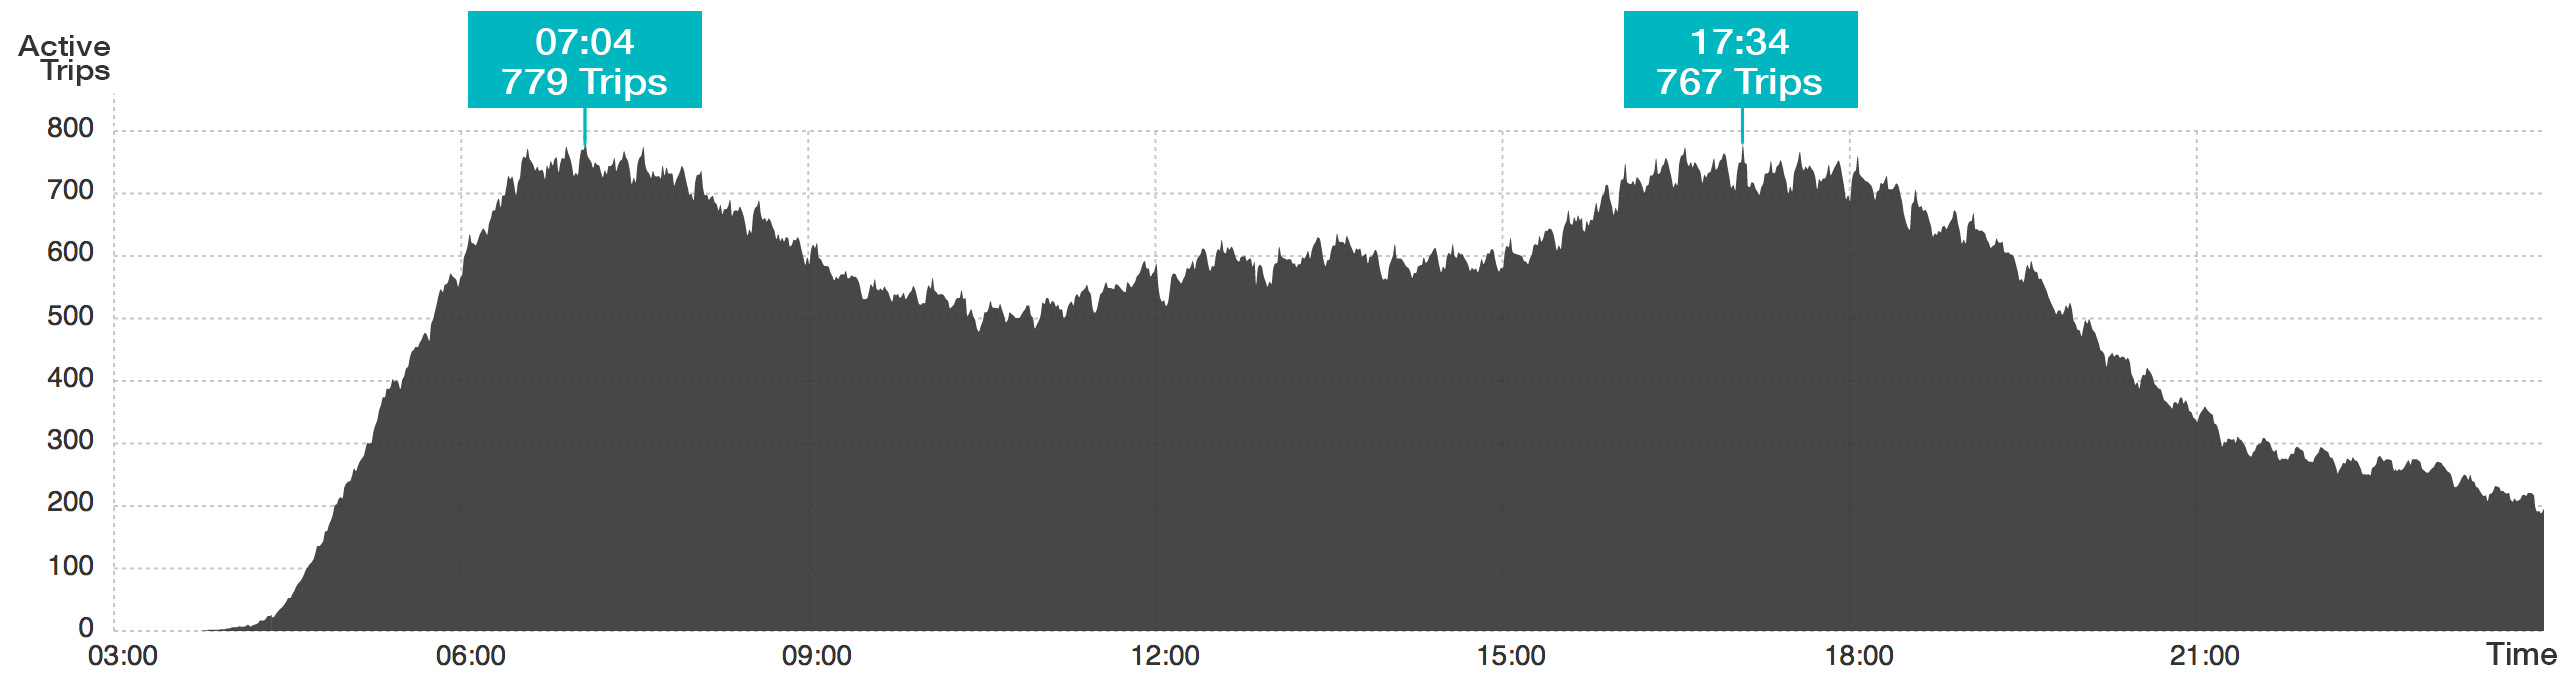
\includegraphics[width=\textwidth]{activeTrips.jpg}
          \caption{Anzahl an aktiven Trips zwischen 3.00 und 24.00 Uhr am 02.08.2017}
          \label{fig:activeTrips}
        \end{center}
      \end{figure}

      Für eine interaktive Karte bedeutet dies, dass je nach Tag zwischen 0 und 1000 Trips aktiv sein können. Dies entspricht dann auch der Anzahl an Vehicles die sie auf der Karte bewegen und animiert werden müssen. Damit dies möglich ist wurde nach Software Lösungen gesucht, die für solche Datenmassen ausgelegt sind. Für die Karte wird dafür Mapbox eingesetzt. Mapbox verwendet Web-GL (basierend auf OpenGL) und bietet damit die Möglichkeit ein GPU unterstütztes Rendering im Browser zu ermöglichen.\\

      Die Wahl der richtigen Tools ist dabei nur die Grundlage um die Datenmenge zu bewältigenden. Viele weitere Schritte sind notwendig um eine performante Webanwendung zu erstellen. Diese werden in Kapitel \ref{sub:backend} \nameref{sub:backend} und \ref{sub:frontend} \nameref{sub:frontend} ausführlich behandelt.


        
    % subsection bewältigung_der_datenmenge (end)
\end{newpage}
  \begin{newpage}
\section{Implementierung}
\label{sec:implementierung}
  In dieser Arbeit wird ein Macbook Pro 2,9 GHz Intel Core i5 mit 16 GB 1867 MHz DDR3 und Intel Iris Graphics 6100 1536 MB eingesetzt.
  Für das Backend wird die Datenbank PostgreSQL und Nodejs verwendet. Nodejs ist nicht nur einfach aufzusetzen, sondern auch sehr performant und effizient für Web Applikationen einsetzbar. Zudem lässt es sich sehr einfach mittels Docker in der AWS (Amazon Web Services) Cloud veröffentlichen.\\

  Dieses Kapitel ist in zwei Abschnitte unterteilt. Namentlich \texttt{Backend} und \texttt{Frontend} genannt. Im Abschnitt Backend sollen die Implementierungsschritte für das Erstellen eines Backends beschrieben werden, dass ein GTFS-Feed verarbeiten und dessen Daten dem Frontend zur Verfügung stellt. Der Abschnitt Frontend beschreibt verschiedene Performance optimierungen und die einzelnen UI-Komponente mit deren Funktionensweise.

  \subsection{Backend}
\label{sub:backend}
  Da der GTFS Standard eine fertige relationale Beziehung der einzelnen Dateien festlegt, ist der Einsatz einer relationalen Datenbank sehr naheliegend. Dabei gibt es eine breite Palette an Auswahl. Damit die Anwendung möglichst Zugänglich bleibt, liegt der Fokus auf Datenbanken die unter einer Open-source Lizenz kostenfrei zur Verfügung stehen. Die zwei populärsten sind MySQL und PostgreSQL\parencite{db_engines}. Beide haben ihre Vor- und Nachteile und die Entscheidung ist mehr eine persönliche Präferenz, als ein großer Vorteil des Einen über den Anderen. Einen kleinen Vorteil bietet PostgreSQL's Unterstützung für Array-Types, welche sehr hilfreich beim speichern und abfragen von Daten ist. Ansonsten ist dieses Projekt auch mit MySQL realisierbar.\\

  In diesem Abschnitt soll beschrieben werden, welche Probleme beim Arbeiten mit dem GTFS Datenformat und einer PostgreSQL Datenbank bestehen und wie diese gelöst sind. Dabei steht vor allem die Behebung von Engpässen bei der Query\footnotemark Performance, als auch die Verringerung der zu verarbeitenden Datenmenge. Sektion \ref{ssub:gtfs_probleme_und_herausforderungen} beschreibt die generelle Problematik, dass durch die Verwendung des GTFS Formats im Backend entsteht. Die folgenden Abschnitte fokussieren sich darauf dieses Problem zu lösen. Abschnitt "`\nameref{ssub:gtfs_optimierungen}"' zeigt verschiedene GTFS Optimierungsschritte. Darauf folgt die Verbesserung von Polylines in Abschnitt \ref{ssub:polyline_optimieren} und endet mit der Denormalisierung von Datenbanktabellen im letzten Abschnitt \ref{ssub:denormalisierung_der_datenbank}.

  \footnotetext{Ein Query ist eine Informationsanfrage an eine Datenbank} 
  
  % Gliederung eventuell nochmals beschreiben.

  \subsubsection{GTFS - Probleme und Herausforderungen}
\label{ssub:gtfs_probleme_und_herausforderungen}
   Bereits 1993 stellte \texttt{Jakob Nielsen} einen Richtwert für die Antwortzeit einer schnellen Webanwendung vor:

  \begin{quote}
    \textit{"`1.0 second is about the limit for the user's flow of thought to stay uninterrupted, even though the user will notice the delay. Normally, no special feedback is necessary during delays of more than 0.1 but less than 1.0 second, but the user does lose the feeling of operating directly on the data."'}\parencite{nielsen}
  \end{quote}

  Ob oder wie dies Antwortzeit erreicht werden kann, soll hier nicht vertieft werden, denn zu diesem Thema habe ich bereits meine Bachelorarbeit gewidmet\parencite{lorer}.

  Damit eine Webanwendung aber überhaupt eine Chance hat, diese Geschwindigkeitsmarke zu erreichen, ist eine schnelle Antwortzeit des Backends sehr wichtig. Dabei sind Antwortzeiten Innerhalb von 0 bis 200 Millisekunden ein sehr guter Wert. Natürlich gilt: Je weniger umso besser. Diese Benchmark mit dem GTFS Format zu erreichen war eine der Hauptherausforderungen dieser Arbeit.\\

  Das GTFS Format hat den entscheidenden Nachteil, dass es eine hohe Komplexität aufweist, sobald Daten aus verschiedenen Tabellen benötigt werden. Für eine Live Visualisierung, sind Daten aus nahezu allen Tabellen relevant. Abbildung~\ref{fig:gtfs_joined_tables} zeigt, welche davon benötigt - beziehungsweise nicht benötigt werden (grau).

  \begin{figure}[ht]
    \begin{center}
      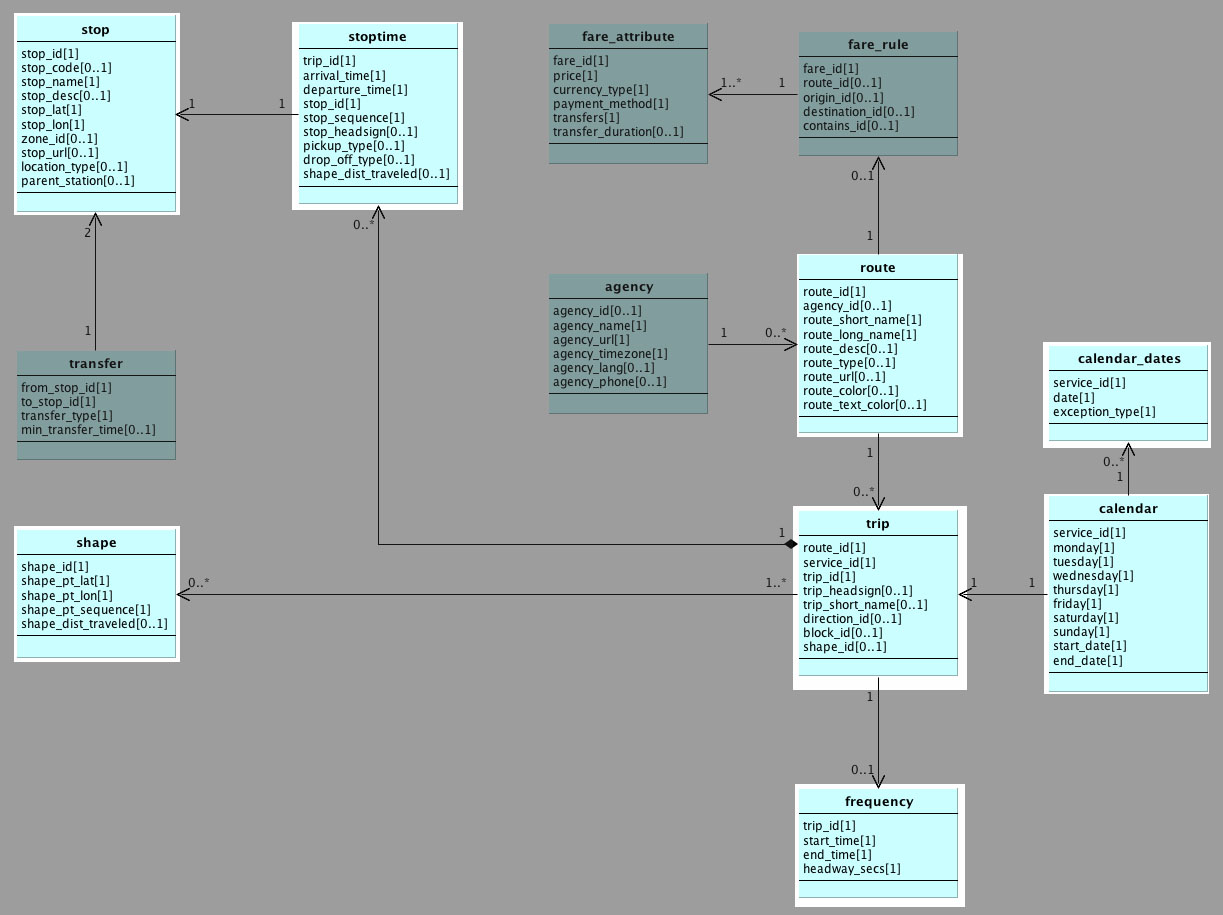
\includegraphics[width=\textwidth]{gtfs_joined_tables.jpg}
      \caption{Benötigte GTFS Tabellen\parencite{google_gtfs_reference}}
      \label{fig:gtfs_joined_tables}
    \end{center}
  \end{figure}

  Das UML Diagramm ist auf den ersten Blick relativ simpel zu verstehen und die Grundlagen der verschiedenen Relationen wurde bereits in Kapitel~\ref{ssec:gtfs_datenformat} beschrieben. Wo liegt also das Problem? In Worten ließe sich diese Datenbankabfrage mit folgendem Statement beschreiben: 

  \begin{quote}
    \label{query_statement}
    \textit{"`Gib uns alle aktiven Trips mit deren Linienverlauf, die am heutigen Tag aktiv sind und in einer Zeitspanne zwischen $t_a$ und $t_b$ liegen."'}
  \end{quote}

  Das große Problem dieses Satze liegt in der Zeitkomponente \textit{"`Trips die am heutigen Tag aktiv sind zwischen ..."'}. Die Trip Tabelle selbst (bezogen auf Abbildung~\ref{fig:gtfs_joined_tables}), hat dies bezüglich keinerlei Informationen darüber. Auch die Calendar- und Calendar-Dates Tabelle beinhaltet nur Informationen, an welchem Datum ein Trip stattfindet, nicht aber um welche Uhrzeit. 

  Erst die Stoptime Tabelle ermöglicht es uns, eine Aussage zu treffen, wann ein Trip aktiv ist. Über die zwei Felder \texttt{arrival\_time} und \texttt{departure\_time} lässt sich sagen, zu welchem Zeitpunkt ein Vehicle an einer Station anhält. Die erste und letzte Station ($S_1$ und $S_n$) geben uns also einen zeitlichen Rahmen, in dem der Trip aktiv ist.
  Hierbei wird klar, dass allein die Beantwortung der Frage zur zeitlichen Komponente, bereits sehr viele Daten aus verschiedenen Tabellen benötigt. Die anderen Tabellen wie \texttt{shape}, \texttt{route}, \texttt{stop} und \texttt{frequency} würden für weitere Informationen wie Vehicle Farbe, Stop Position (Längen- und Breitengrad) oder den Linienverlauf (shape) benötigt werden. Um an die Daten zu gelangen, müssen alle benötigten Tabellen mittels SQL \texttt{JOIN} miteinander verknüpft werden. Dies geschieht durch die Verbindung der einzelnen Reihen zweier Tabellen (TabelleA und TabelleB) gegen eine Verknüpfungsbedingung. Das Resultat ist eine neue Ergebnistabelle mit den Inhalten der kombinierten Reihen. Solche Verknüpfungen sind besonders dann Zeitintensiv, wenn eine große Menge an Daten (siehe Tabelle:~\ref{table:table_metrics}) kombiniert werden. Die Metriken der Tabellen sind dabei wie folgt:

  \begin{longtable}{|>{\raggedright \arraybackslash}p{5.0cm}|>{\raggedright \arraybackslash}p{5.0cm}|>{\raggedright \arraybackslash}p{5.0cm}|}
  \caption{Tabellen Metriken} \label{table:table_metrics}\\
    \hline
    Tabellen Name & Anzahl Reihen\\
    \hline
    trips.txt & 71,000\\
    stop\_times.txt & 1,3000,000\\
    stops.txt & 7,900\\
    shapes.txt & 1,085,860\\
    \hline
  \end{longtable}
  
  Die für das oben genannte Statement~\ref{query_statement} äquivalente SQL-Abfrage ist aufgrund seiner Länge (113 Zeilen Code) im Anhang unter Listing~\ref{lst:get_active_trips_query} zu finden. Diese SQL Abfrage ist allerdings nicht Performant. Sollen alle Trips in einem Zeitraum von 1 - 15 Minuten gefunden werden, sind bereits Rechenzeiten entstanden, die aufgrund ihrer langen Laufzeit abgebrochen werden mussten. In mehreren Iterationen wurde versucht die SQL-Abfrage zu optimieren, was allerdings keine Verbesserung herbeiführte. Es sind zu viele JOIN Verknüpfungen und WHERE Bedingungen in dieser Abfrage, als das sich eine Performante Lösung damit finden lässt. Es musste ein neuer Ansatz gefunden werden um Abfragezeiten erheblich zu verringern.
  
% subsubsection gtfs_probleme_und_herausforderungen (end)
  \subsubsection{GTFS Optimierungen}
\label{ssub:gtfs_optimierungen}

  Der erste Schritt um die Performance zu verbessern, ist die Optimierung von GTFS Feeds. Damit lässt sich die Datenmenge bereits vor dem Importieren in die Datenbank, erheblich verringern. Ein Tool um ein GTFS Feed umfassend zu optimieren ist \texttt{gtfstidy} \url{https://github.com/patrickbr/gtfstidy}. Es bietet dabei allerdings nicht nur die Möglichkeit für die Vereinfachung von Polylines sondern kommt mit einer ganzen Reihe an Optimierungsmöglichkeiten. 

  Der Kommandozeilenbefehl \colorbox{materialGrey}{\texttt{\color{white}{\$ gtfstidy -sSiRDeO input.zip output}}} optimiert das Stuttgart-VVS Feed wie folgt:
  
  \begin{itemize}[label={}]
    \item \textbf{-s} Reduziert die Punktanzahl einer Polyline
      
    \item \textbf{-S} Entfernt redundante Polylines.

    \item \textbf{-i} Umwandlung von Zeichen ID's (String) in Zahlen ID's (Integer).\footnote{Aus der String ID \texttt{'1.T0.10-1-j17-1.16.H'} wird \texttt{78}}

    \item \textbf{-O} Entfernt Feed Einträge die nicht referenziert werden.

    \item \textbf{-R} Entfernt doppelt vorhandene Routen.

    \item \textbf{-e} Setzt fehlerhafte oder optionale Felder auf einen Standard Wert.

    \item \textbf{-D} Entfernt fehlerhafte Einträge aus dem Feed.
  \end{itemize}

  Durch Verwendung von gtfstidy konnte das Feed optimiert werden und die Datengröße der einzelnen Dateien um folgendes Maß verringert werden.

  \begin{longtable}{|>{\raggedright \arraybackslash}p{5.0cm}|>{\raggedright \arraybackslash}p{5.0cm}|>{\raggedright \arraybackslash}p{5.0cm}|}
    \hline
    Dateiname & Größe davor& Größe danach\\
    \hline
    trips.txt & 6 MB & 2.8 MB\\
    stop\_times.txt & 103 MB & 53 MB\\
    stops.txt & 651 KB & 355 KB\\
    shapes.txt & 77.3 MB & 22.4 MB\\
    routes.txt & 54 KB & 38 KB\\
    calendar\_dates.txt & 557 KB & 463 KB\\
    \hline
    \caption{Tabellengröße bevor und nach anwenden von gtfstidy}
    \label{tbl:gtfs_tidy_results}
  \end{longtable}

  Insgesamt konnte so die Größe des Feeds von 79 MB auf 118 MB um knapp 50\% verringert werden. Vor allem die Umwandlung von langen String ID's in kürzere Integer ID's trägt maßgeblich zur Verringerung der Dateigröße bei.

% subsubsection gtfs_optimierungen (end)
  \subsubsection{Polyline optimieren}
\label{ssub:polyline_optimieren}

  Die Optimierung der Polyline ist ein sehr wichtiger Aspekt in meiner Arbeit und soll in diesem Abschnitt vertieft werden.

  \subsubsection*{Ramer–Douglas–Peucker}
  \label{ssub:ramer_douglas_peucker}
    Das Problem: Die im Stuttgart-VVS Feed zur Verfügung gestellten Polylines sind Überdefiniert und können aus tausenden Punkten bestehen. Für eine Visualisierung ist eine solche Genauigkeit nicht notwendig und aufgrund der großen Datenmenge problematisch. Im vorigen Abschnitt \ref{ssub:gtfs_optimierungen} wurde die Option \colorbox{materialGrey}{\texttt{\color{white}{-s}}} vorgestellt. Dieser Befehl verwendet den "`Ramer–Douglas–Peucker"' (RDP) Algorithmus um die Anzahl der Punkte einer Polyline zu reduzieren. Der Vorteil besteht darin, dass dabei nicht der Linienverlauf verändert wird. Abbildung~\ref{fig:simplify} zeigt ein Beispiel einer solchen Vereinfachung mittels einer JavaScript Bibliothek\footnote{Simplify.js \url{http://mourner.github.io/simplify-js/}}.

    \begin{figure}[htbp]
      \centering
      \subfloat[Polyline vor RDP]{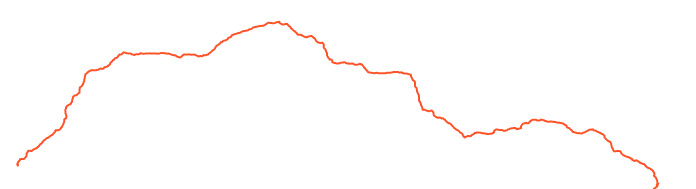
\includegraphics[width=0.48\textwidth]{simplify_before.jpg}\label{fig:simplify_before}}
      \hfill
      \subfloat[Polyline nach RDP]{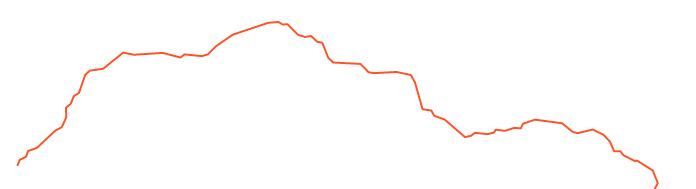
\includegraphics[width=0.48\textwidth]{simplify_after.jpg}\label{fig:simplify_after}}
      \caption{Vereinfachung einer Polyline mittels Simplify.js}
      \label{fig:simplify}
    \end{figure}

    Ausgangspunkt ist eine Polyline mit $\approx1000$ Punkten (\ref{fig:simplify}a). Nach der Vereinfachung (\ref{fig:simplify}b) ist die Anzahl auf 100 Punkte reduziert, ohne dabei visuell merklich einzubüßen. Dies ist eine erhebliche Reduzierung der Punkte um 90\%. Wie wirkt sich dieser Algorithmus positiv auf das Projekt aus? Die Vorteile sind weitreichend. Sehen wir uns die Shape Tabelle in Abbildung \ref{fig:shape_simplify} an. \ref{fig:shape_simplify}a zeigt 394 Reihen vor der Optimierung und nur noch 140 (\ref{fig:shape_simplify}b) nach Anwendung von gtfstidy.

    \begin{figure}[htbp]
      \centering
      \subfloat[Shapte Tabelle vor RDP]{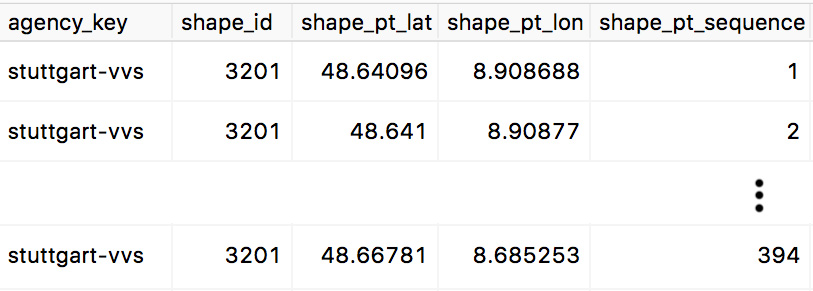
\includegraphics[width=0.48\textwidth]{shape_simplify_before.jpg}\label{fig:shape_simplify_before}}
      \hfill
      \subfloat[Shapte Tabelle nach RDP]{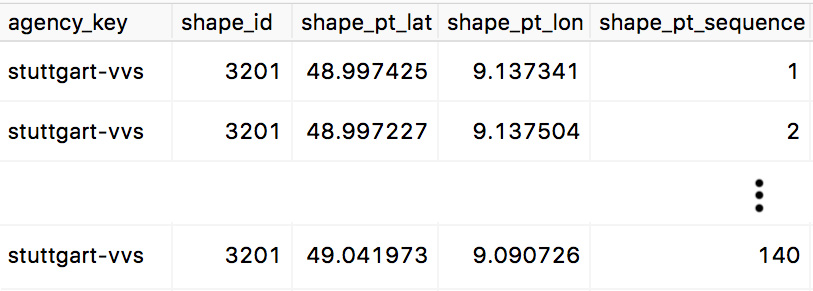
\includegraphics[width=0.48\textwidth]{shape_simplify_after.jpg}\label{fig:shape_simplify_after}}
      \caption{Reduzieren der Polyline via gtfstidy}
      \label{fig:shape_simplify}
    \end{figure}

    In seinem Originalzustand hat das verwendete VVS Feed 1,085,859 Mio Zeilen. Nach der Anwendung sind diese auf 617,653 Tsd. verringert. Testet man folgende PostgreSQL Abfrage
    \colorbox{materialGrey}{\texttt{\color{white}{{\color{materialBlue}SELECT} * {\color{materialBlue}FROM} gtfs\_shapes {\color{materialBlue}WHERE} shape\_id = {\color{materialRed}3201}}}}
    die alle Punkte einer Polyline ausgeben soll, so ergibt sich für ein optimiertes Feed eine Query Zeit von $\approx145 ms$ und für das nicht optimierte Feed $\approx250 ms$. Schon durch diese einfache Methode sind bereits erste Performance Steigerungen wahrnehmbar.

  % subsubsection ramer_douglas_peucker (end)

  \subsubsection*{Aggregieren der Shape Tabelle}
  \label{ssub:aggregieren_der_shape_tabelle}
    In GTFS wird für jeden Punkt einer Polyline eine Reihe in der Datenbank belegt. Diese Abfolge ist durch eine sogenannte \texttt{Shape Point Sequence} festgelegt, was nichts anderes ist als eine Zahl von $1$ bis $n$. Dies ist auch bereits in obiger Tabelle \ref{fig:shape_simplify} zu sehen gewesen. Sehr viel effektiver wäre es allerdings, diese Punkte nicht Reihenweise zu speichern, sondern alle zusammen gehörenden Punkte in einem einzigen Feld zu speichern. Dies ist in PostgreSQL durch eine Aggregierung möglich. Daraus ergibt sich folgende Shape Tabelle:

    \begin{figure}[htbp]
      \begin{center}
        
\includegraphics[width=\textwidth]{aggregated.png}
        \caption{Aggregierte Koordinaten der Shape Tabelle}
        \label{fig:aggregated}
      \end{center}
    \end{figure}

    Wie zu sehen ist benötigt nun eine Polyline in der Shape Tabelle nicht mehr 140 Reihen, sondern nur noch eine einzige. Für diese Arbeit ist dies auf alle Polylines angewendet worden und in einer neuen Tabelle namens \texttt{denormalized\_shapes} abgespeichert. Dadurch ist die Berechnung der Aggregierung nur einmal nötig. Der SQL-Befehl dafür ist dem Anhang unter \ref{lst:sql_aggregate_shape}. zu entnehmen.
    Wenden wir die selbe SQL Abfrage, die bereits oben Verwendung fand, auf die neue \texttt{denormalized\_shapes} Tabelle an. Die Query Zeit ist auf $\approx1ms$ gesunken! Anstatt hunderte Reihen muss nur eine einzige Reihe ausgelesen werden, was sehr sehr schnell ist. Durch das Denormalisieren\footnotemark der Shape Tabelle ist auch die Anzahl der Reihen auf ein Minimum gesunken. Von den früheren 617,653 Tsd. Reihen, sind jetzt durch die Aggregation nur noch 4,524 Tsd. übrig.

    \footnotetext{Denormalisieren beschreibt den Prozess der Relationsauflösung von Datenbanktabellen.}
  
  % subsubsection aggregieren_der_shape_tabelle (end)

  \subsubsection*{Polyline Encoding}
  \label{ssub:polyline_encoding}
    Die letzte Maßnahme zur Optimierung der Polyline stellt das sogenannte Polyline Encoding dar. Wie dieses Verfahren genau funktioniert, geht an dieser Stelle zu weit. Hier soll nur erklärt werden, was das Polyline Encoding für diese Arbeit bedeutet und warum es verwendet wird.\\

    Das Polyline Encoding kann in JavaScript beispielsweise durch das Google-Polyline\footnote{\url{https://www.npmjs.com/package/google-polyline}} Paket eingesetzt werden. Das Encoding wandelt eine Polyline, bestehend aus Punkten, in einen String um. Zum Beispiel die Punkte: (38.5, -120.2), (40.7, -120.95), (43.252, -126.453) werden als
    \colorbox{materialGrey}{\texttt{\color{white}{\_p\textasciitilde iF\textasciitilde ps|U\_ulLnnqC\_mqNvxq`@}}}
    codiert. Dies geschieht in meiner Anwendung immer genau dann, bevor Daten von Server in Richtung Client geschickt werden: Encode $\rightarrow$ Send $\rightarrow$ Decode. Da eine codierte Polyline weniger Zeichen benötigt, kann damit Datenvolumen bei der Kommunikation zwischen Server und Client gespart werden.

  % subsubsection polyline_encoding (end)


% subsubsection polyline_optimieren (end)
  \subsubsection{Denormalisierung der Datenbank}
\label{ssub:denormalisierung_der_datenbank}
  Die Denormalisierung ist eine Strategie, die auf eine zuvor normalisierte Datenbank angewendet wird, um die Leistung zu erhöhen. Die Denormalisierung ist der Prozess, bei dem versucht wird, die Leseperformance einer Datenbank zu verbessern, auf Kosten der Schreibleistung, durch Hinzufügen redundanter Kopien von Daten oder durch deren Gruppierung.\parencite{sanders}
  Der große Nachteil von Denormalisierung, nämlich die Redundanz von Daten, spielt für dieses Projekt keine Rolle, da die Daten ausschließlich ausgelesen und nicht geschrieben werden. Was bleibt sind die Vorteile.\\

  Für dieses Projekt bedeutet diese Methode, eine neue Tabelle zu generieren, die den Zugriff auf die benötigten Daten einfach macht. Im Grunde handelt es sich um eine Vorberechnung. Anstatt die Tabellen bei jeder Anfrage an den Server aufwendig über viele \texttt{SQL-JOINS} zu verknüpfen, wird diese Verknüpfungen einmalig vorberechnet und in eine Tabelle gespeichert. Eine Denormalisierung  einer Tabelle ist bereits im vorherigen Abschnitt "`\nameref{ssub:aggregieren_der_shape_tabelle}"' gezeigt und führte dazu, dass die Polyline über die Abfrage einer einzigen Tabellenreihe erhalten werden kann was die Performance signifikant erhöhte. Zur besseren Verständnis soll folgende Grafik helfen:

  \begin{figure}[htbp]
    \begin{center}
      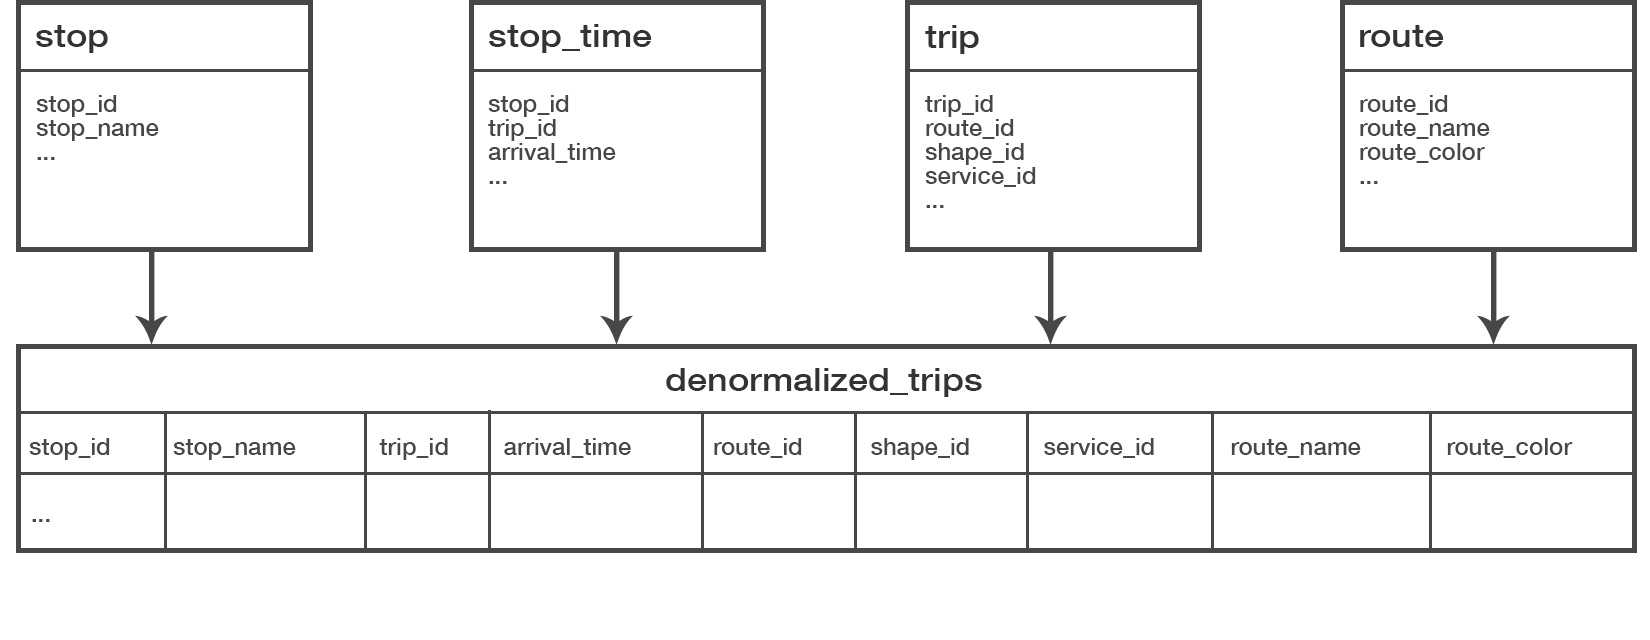
\includegraphics[width=\textwidth]{denormalizing.jpg}
      \caption{Beispiel einer Denormalisierung von Tabellen}
      \label{fig:denormalizing}
    \end{center}
  \end{figure}

  Wie in Abbildung \ref{fig:denormalizing} zu sehen ist, wird aus einer vertikalen Anordnung der einzelnen Datenfelder, eine horizontale Anordnung in einer einzigen \texttt{denormalized\_trips} Tabelle. Eine Reihe in dieser neuen Tabelle steht für genau einen Eintrag eines Trips. Anstatt also bei jeder Anfrage an den Server die verschiedenen Daten mittels \texttt{JOIN} verknüpfen zu müssen, können diese jetzt per Zugriff auf eine einzige Reihe in nur einer Tabelle erfragt werden.\\

  Dieses Prinzip, der Gruppierung von Daten in einer neuen Tabelle soll nun auch auf die anderen benötigten Tabellen angewendet werden. Die Denormalisierung erfolgt in 3 Schritten:

  \begin{enumerate}
    \item Erstellen der neuen Tabelle \texttt{denormalized\_trips}
    \item Importieren der verschiedenen Daten in diese neue Tabelle
    \item Mögliche Abfragen sind nun über diese neue Tabelle möglich.
  \end{enumerate}

  Das SQL-Statement ist abermals aufgrund seiner Länge Anhang \ref{lst:denormalized_shapes} zu entnehmen. Dies resultiert in einer Tabelle die wie folgt aussieht:

  \begin{figure}[htbp]
    \begin{center}
      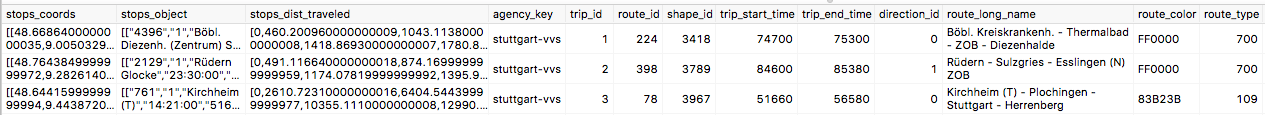
\includegraphics[width=\textwidth]{denormalized_tables.png}
      \caption{Auszug aus der \texttt{denormalized\_trips} Tabelle}
      \label{fig:denormalized_table}
    \end{center}
  \end{figure}  

  \subsubsection*{Ergebnisse der Denormalisierung}
  \label{ssub:ergebnisse_der_denormalisierung}
    Für die Visualisierung ist eine Abfrage der aktiven Trips am wichtigsten.
    Folgende Tabellen werden für die Abfrage benötigt.

    \begin{figure}[htbp]
      \begin{center}
        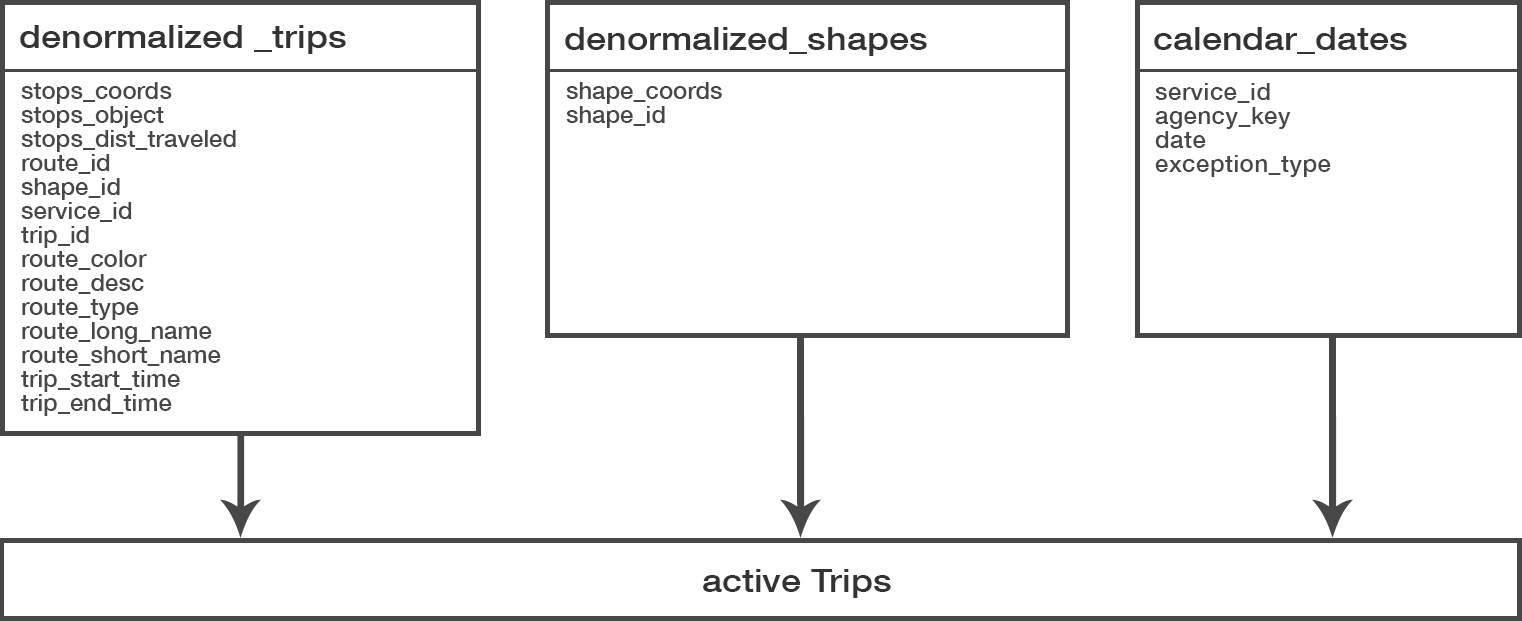
\includegraphics[width=\textwidth]{denormalizing_results.jpg}
        \caption{Benötigte Tabellen zur Abfrage von Trips}
        \label{fig:denormalizing_results}
      \end{center}
    \end{figure}

    Wie zu sehen ist, wird auf die Denormalisierte \texttt{Shape} und \texttt{Trips} Tabelle zugegriffen.

    Nachfolgend die Ergebnisse für die Abfrage von Trips in einem wachsenden Zeitrahmen. Die verwendete SQL-Abfrage befindet sich im \nameref{sec:anhang} unter Listing \ref{lst:query_trips}.

    \begin{longtable}{|>{\raggedright \arraybackslash}p{5.0cm}|>{\raggedright \arraybackslash}p{5.0cm}|>{\raggedright \arraybackslash}p{4.0cm}|}
    \caption{Evaluierung der Denormalisierung}\label{tbl:evaluierung_der_denormalisierung}\\
      \hline
        Zeitraum & Trip Anzahl & Query Zeit\\
      \hline
        9:00 bis 9:15 & 88 & 98 ms\\
        9:00 bis 10:00 & 1125 & 154 ms\\
        9:00 bis 12:00 & 3360 & 285 ms\\
        9:00 bis 15:00 & 7070 & 497 ms\\
        9:00 bis 21:00 & 14718 & 900 ms\\
      \hline
    \end{longtable}

    Die Ergebnisse Zeigen, dass die Abfragezeit der Datenbank für die aktiven Trips erheblich gesunken ist. Anfangs ist solch eine Anfrage aufgrund der endlosen Laufzeit erst gar nicht möglich gewesen.

    \pagebreak 

    \begin{figure}[htbp]
      \begin{center}
        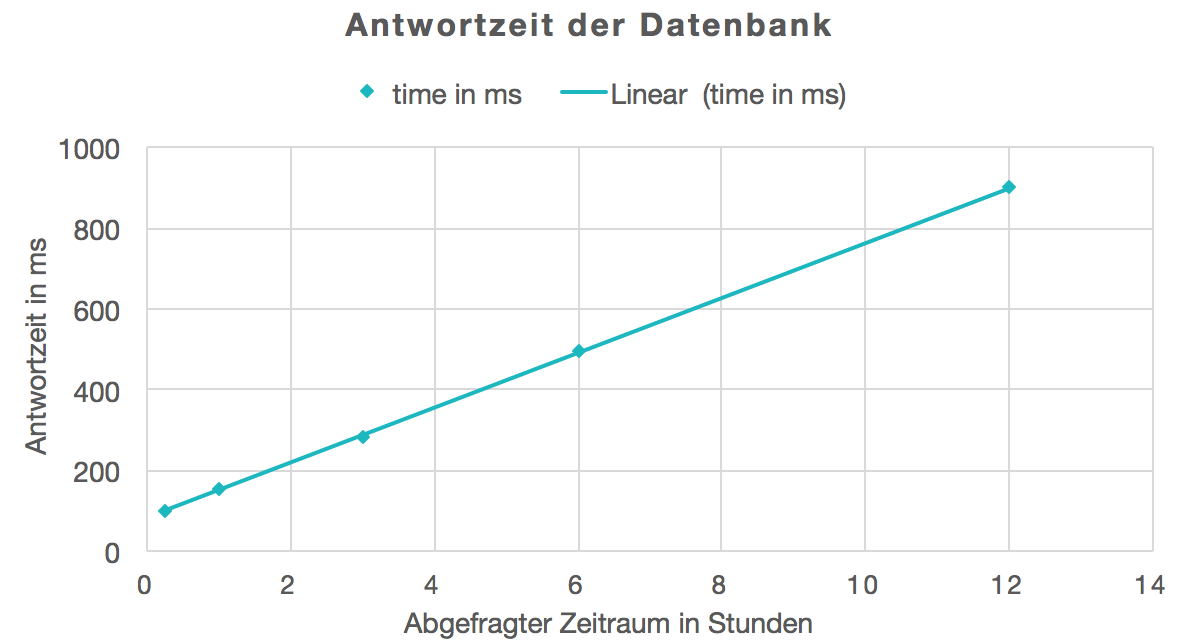
\includegraphics[width=0.65\textwidth]{query_time_chart}
        \caption{Plot der Abfragezeiten}
        \label{fig:query_time_chart}
      \end{center}
    \end{figure}
    
    Abbildung \ref{fig:query_time_chart} zeigt einen Plot der Query Zeit aus Tabelle \ref{tbl:evaluierung_der_denormalisierung} als nahezu linearen Graphen. Daraus folgt, dass die Antwortzeit der Datenbank linear mit dem abgefragten Zeitraum wächst. In der Visualisierung sind vor allem Trip Abfragen zwischen einer Minute und einer Stunde in Verwendung. Die Abfragezeit bewegt sich damit zwischen $\approx 80 -  160\; ms$.
    
  % subsubsection ssub:ergebnisse_der_denormalisierung (end)

% subsubsection denormalisierung_der_datenbank (end)
  \subsubsection{API Endpunkte}
\label{ssub:api_endpunkte}
  Um einen Datenaustausch zwischen Server und Client zu ermöglichen, sind folgende API\footnotemark Endpunkte vorhanden. 

  \footnotetext{Application Programming Interface}

  \begin{itemize}[label={}]
    \item \textbf{/daily} Stellt die Daten für das Zeitstrahldiagramm bereit. Wird beim Start der Anwendung einmalig Angefragt. Die Antwort enthält XY-Wertpaare. X stellt dabei die Zeit in Sekunden und Y die zu diesem Zeitwert aktiv werdenden Trips dar.

\begin{lstlisting}[captionpos=t, caption=Antwort des Servers zur Anfrage \texttt{/daily}, label=lst:daily_response]
[
  {"x":86340,"y":"6"},
  {"x":86400,"y":"10"}, 
  ...
]
\end{lstlisting}

    \item \textbf{/trips/:from,:to} Ermöglicht das Abfragen von Trips, die in einer Zeitspanne \texttt{from - to} aktiv sind. Beim initialen Aufruf der Webanwendung wird dieser Endpunkt als erstes angefragt um die aktiven Trips innerhalb einer Stunde zu bekommen. Der gewählte Zeitraum ist in Sekunden anzugeben. Die Definition ist wie folgt: $t_{from} = now$ und $t_{to} = now + 600 sec$. Die Sekunden lassen sich nach der Formel aus Kapitel \ref{ssub:time} berechnen.
     durch das Addieren der Stunden, Minuten und Sekunden errechnen. Bsp: 17:04:59 Uhr

    $\Rightarrow t_{from} = 61499 \Rightarrow t_{to} = 61499 + 600\;sec$ $\Rightarrow$ \texttt{/trips/61499,62099}

    Die Antwort des Servers auf einen Endpunkt vom Typ \texttt{/trips/} ist ein Objekt mit der Trip\_Id, dessen Inhalt der \texttt{GeoJSON} spezifikation nach RFC 7946 folgt:

\begin{lstlisting}[captionpos=t, caption=Trip Objekt, label=lst:trip_object]
{
  2498: {  
    "type": "FeatureCollection",
    "features": [
      {
        "type": "Feature",
        "properties": {
          "name": "shape",
          ...
        },
        "geometry": {
          "type": "LineString",
          "coordinates": [[9.4437,48.64482], ...]
        }
      },
      {
        "type": "Feature",
        "properties": {
          "name": "station"
        },
        "geometry": {
          "type": "Point",
          "coordinates": [9.443688, 48.6448]
        }
      },
      ...
    ]
  }
}
\end{lstlisting}
  
    Da die Antwort in Listing \ref{lst:trip_object} mittels "`..."' gekürzt ist, sind detailiertere Antworten im \nameref{sec:anhang} unter Listing \ref{lst:geojson_featurecollection}, \ref{lst:shape_feature} und \ref{lst:station_feature} zu finden.
  

    \item \textbf{/trips/:id} Antwortet mit den zur ID gehörenden Trip Informationen. Dieser Endpunkt ermöglicht es, Informationen für nur einen einzigen Trip zu bekommen. Dies ist vor allem dann hilfreich, wenn der Nutzer ein Vehilce anklickt und Informationen über diesen Trip angezeigt bekommen möchte. Beispiel: \texttt{/trips/51295}

    \item \textbf{/trips/new/:from,:to,:tripIds} Stellt die Abfrage für neue Trips zur Verfügung und exkludiert dabei diejenigen Trips, die in \texttt{:tripIds} genannt sind. Damit wird verhindert, dass bereits auf der Karte vorhandene Trips nicht doppelt auftauchen können. Dieser Query wird in einem 30 Sekunden Intervall vom Client an den Server gesendet um die neusten Trips zu erhalten. Damit wird die Karte aktuell gehalten. Beispiel: Es ist 10:00 Uhr, hole die in der nächsten Minute aktiv werdenden Trips (Zeitraum 10:00 bis 10:01 Uhr) und schließe die Trips mit der ID \texttt{51295,9212,52} vom Ergebnis aus \texttt{/trips/new/36000,36060,51295,9212,52}.

    \item \textbf{/trips/new/:from,:to} Stellt die gleiche Funktionalität wie der vorherige Endpunkt zur Verfügung, mit der Ausnahme, dass keine Trip-ID's übermittelt werden müssen. Dieser Endpunkt ist beispielsweise dafür da, falls die Karte leer ist und noch keine aktiven Trips enthält.

  \end{itemize}

% subsubsection api_endpunkte (end)
  \subsubsection{Server}
\label{ssub:server}
  Der Nodejs Server stellt die zuvor definierten Endpunkte mittels \texttt{Express.js} als ansprechbare Routen dem Client zur Verfügung. Express ist ein minimalistisches Node.js Framework für moderne Web Applikationen. Es vereinfacht die Erstellung von API Endpunkten durch das Bereitstellen hilfreicher Methoden zur Erstellung von Routen\footnotemark.

  \footnotetext{Routing refers to determining how an application responds to a client request to a particular endpoint, which is a URI (or path) and a specific HTTP request method (GET, POST, and so on). \url{https://expressjs.com/en/starter/basic-routing.html}}

  \begin{figure}[htbp]
    \begin{center}
      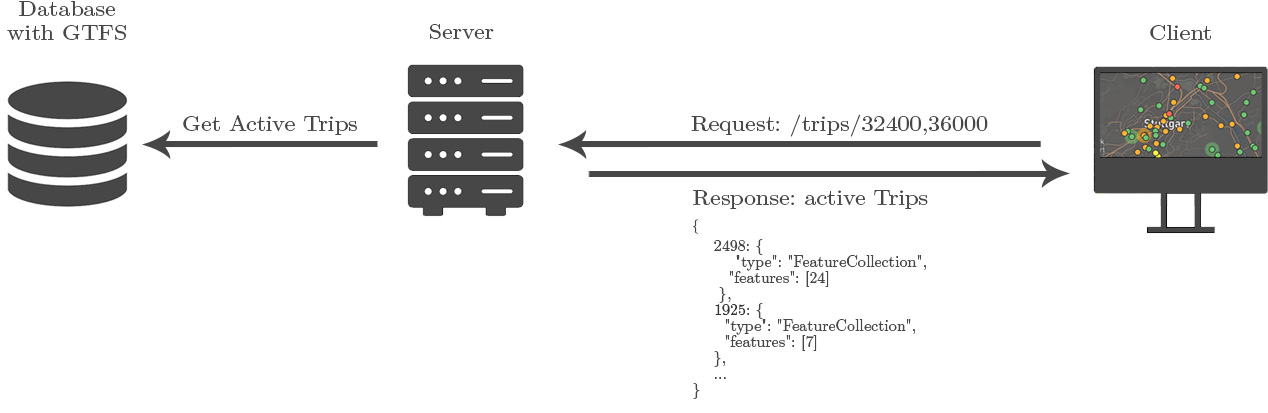
\includegraphics[width=\textwidth]{server_client.jpg}
      \caption{Server / Client Relation}
      \label{fig:server_client}
    \end{center}
  \end{figure}

  Trifft eine valide Anfrage auf den \texttt{/trips/:from,:to} Endpunkt, so wird ein Ablauf nach Abbildung \ref{fig:server_client} angestoßen.
  Die eintreffenden Anfragen werden vom Server entgegengenommen, validiert, verarbeitet und anschließend die entsprechende Antwort zurück gesendet. Die Validierung prüft die vom Client übergebenen Parameter auf ihre Plausibilität. Schlägt diese Prüfung fehl wird ein Fehler vom Server zurückgegeben und der Server wartet auf eine neue Anfrage. Die wichtigste Routine des Servers stellt die Abfrage von Trips aus der Datenbank dar. Die Datenbank sucht diejenigen Trips heraus, welche in dem benötigten Zeitraum \texttt{from, to} aktiv sind. Dabei wird das Datum und der Wochentag zum Zeitpunkt der Anfrage verwendet. Damit der Client bei der Animation möglichst wenig Rechenarbeit hat, werden alle Daten, bei denen dies möglichst ist, vorberechnet. Folgender Ablauf findet statt:

  \begin{itemize}
    \item \textbf{Daten Mapping:} Die Trips aus der Datenbank werden in das \texttt{GeoJSON}-Format umgewandelt, damit diese im weiteren Programmverlauf einfacher zu verarbeiten sind. Dabei werden die im Kapitel "`\ref{sub:begriffe} \nameref{sub:begriffe}"' festgelegten Definitionen beachtet.

    \item \textbf{Zurückgelegte Distanz:} Damit eine Animation der Vehicle stattfinden kann ist die Berechnung der Distanzen zwischen den einzelnen Stationen nötig. Falls das Feld \texttt{stops\_dist\_traveled}\footnotemark in der Datenbank vorhanden ist, kann die zurückgelegte Distanz sehr einfach daraus berechnet werden. Ist dies nicht der Fall so wird ein Station Matching durchgeführt, um die Distanzen berechnen zu können.
    \footnotetext{Die zurückgelegte Distanz bis zu einer Station $S$}

    \item \textbf{Station Matching:} Unter Station Matching versteht sich die Positionierung der Stationen auf und entlang der Polyline. Dies wird im nächsten Abschnitt ausführlicher betrachtet.

    \item \textbf{Feststellen der Richtung:} Für eine Polyline ist es unerheblich ob die Koordinaten in der Reihenfolge $\{ p_1, p_2, \dotsc, p_n \}$ oder $\{ p_n, \dotsc, p_2, p_1 \}$ angeordnet sind. Damit das Vehicle aber in die richtige Richtung von $A$ nach $B$ fährt, ist es wichtig dass die Koordinaten der Polyline in aufsteigender Reihenfolge festgelegt werden. Falls dies nicht er Fall ist, werden die Koordinaten in ihrer Reihenfolge umgekehrt.

    \item \textbf{Codieren der Polyline:} Zuletzt werden die Koordinaten in einen Polyline String Codiert und abschließend versendet.
  \end{itemize}

  \input{sections/implementation/backend/station_matching}

% subsubsection server (end)
  \subsubsection{Backend Performance}
\label{ssub:backend_performance}
  In diesem Abschnitt soll das gesamte Backend (Server und Datenbank) evaluiert werden. Dazu werden sowohl die Zeit zum Abfragen der Datenbank, als auch die Zeit zur Datenverarbeitung auf dem Server betrachtet werden.

  \begin{longtable}{|>{\raggedright \arraybackslash}p{4.5cm}|>{\raggedright \arraybackslash}p{1.2cm}|>{\raggedright \arraybackslash}p{1.2cm}|>{\raggedright \arraybackslash}p{1.2cm}|>{\raggedright \arraybackslash}p{1.2cm}|>{\raggedright \arraybackslash}p{1.2cm}|>{\raggedright \arraybackslash}p{1.2cm}|}
  \caption{Backend Evaluation}\label{tbl:backend_evaluation}\\
    \hline
    Anz. Trips & 20 & 100 & 500 & 1000 & 5000 & 10000\\
    \hline
    Query Zeit (ms)        & 25 & 88 & 124 & 200 & 855 & 1631 \\
    Verarbeitungszeit (ms) & 2 & 27 & 40 & 142 & 226 & 435 \\
    Summe (ms)             & 27 & 115 & 164 & 342 & 1081 & 2066 \\
    \hline
  \end{longtable}

  In Tabelle \ref{tbl:backend_evaluation} sind die Datenwerte für verschiedene Abfragen aufgelistet. Die Werte ergeben sich aus dem Mittelwert der Laufzeit in 10 Durchläufen. Wie bereits in Kapitel "`\nameref{sub:bewältigung_der_datenmenge}"' festgestellt:

  \begin{quote}
    \textit{"`In einer Minute [werden] minimal 0 und maximal 27 Vehicle aktiv. Im Schnitt starten 9 Vehicles pro Minute ihre Fahrt."'}\ref{sub:bewältigung_der_datenmenge}
  \end{quote}

  Aus dieser Aussage plus den gemessenen Werten lässt sich folgende Schlussfolgerung ziehen: Bei einer Anzahl zwischen 20 und 100 Trips reagiert der Server innerhalb von 25 bis $120ms$. Da die meisten Trips in diese Spanne fallen, ist dieses Ergebnis am bedeutendsten. 

  Im Bereich von 100 bis 500 Trips ist eine Antwortzeit von 115 bis $164ms$ immer noch sehr gut. Diese Anzahl an Trips ist dann relevant, wenn die Applikation das erste mal aufgerufen wird und die Karte noch leer ist. In diesem Fall kann es sein, dass der Server (je nach Datum und Uhrzeit) zwischen 200 - 500 Trips verarbeiten muss. Aber selbst Abfragen von bis zu 10.000 Trips, was ungefähr einer Zeitspanne von einem Tag gleich kommt, sind immer noch innerhalb von 2 Sekunden verarbeitet.\\

  Abschließend kann gesagt werden, dass in dieser Arbeit ein performantes Backendsystem für eine Web Applikation entwickelt worden ist, welches Serveranfragen effizient be- und verarbeiten kann.

  % \ref{sub:bewältigung_der_datenmenge}

% subsubsection backend_performance (end)
  % \subsubsection{Konfigurierung}
\label{ssub:konfigurierung}
  \begin{itemize}
    \item Why optimize
    \item what can be optimize
    \item a-b test of configuration
    \item discuss test results
  \end{itemize}
% subsubsection konfigurierung (end)
% subsection backend (end)

  \begin{newpage}
  
  \subsection{Frontend}
  \label{sub:frontend} 
    Das Frontend besteht aus verschiedenen UI-Komponenten. Diese sollen in diesem Kapitel beschrieben und die wichtigsten Algorithmen zur Darstellung der Vehicle werden näher betrachtet.

  \subsubsection{UI Komponenten}
\label{ssub:ui_komponenten}

  In diesem Abschnitt sollen die verschiedenen UI-Komponenten vorgestellt werden.

  \subsubsection*{Die Karte}
  \label{ssub:die_karte}
    Die Karte (\ref{fig:map}) ist standardmäßig auf den Längengrad 9.244 und Breitengrad 48.757 ausgerichtet. Damit findet sich der Anwender beim Aufrufen der Applikation gleich an der richtigen Stelle wieder. Die Karte verwendet eine abgeänderte Version des Kartenstils \texttt{Mapbox-Dark}. Dabei wurden Parks, Grünflächen und Wasser subtil eingefärbt und die Routen des GTFS-Feeds mit einem leichtem Orange hervorgehoben.

    \begin{figure}[htbp]
      \begin{center}
        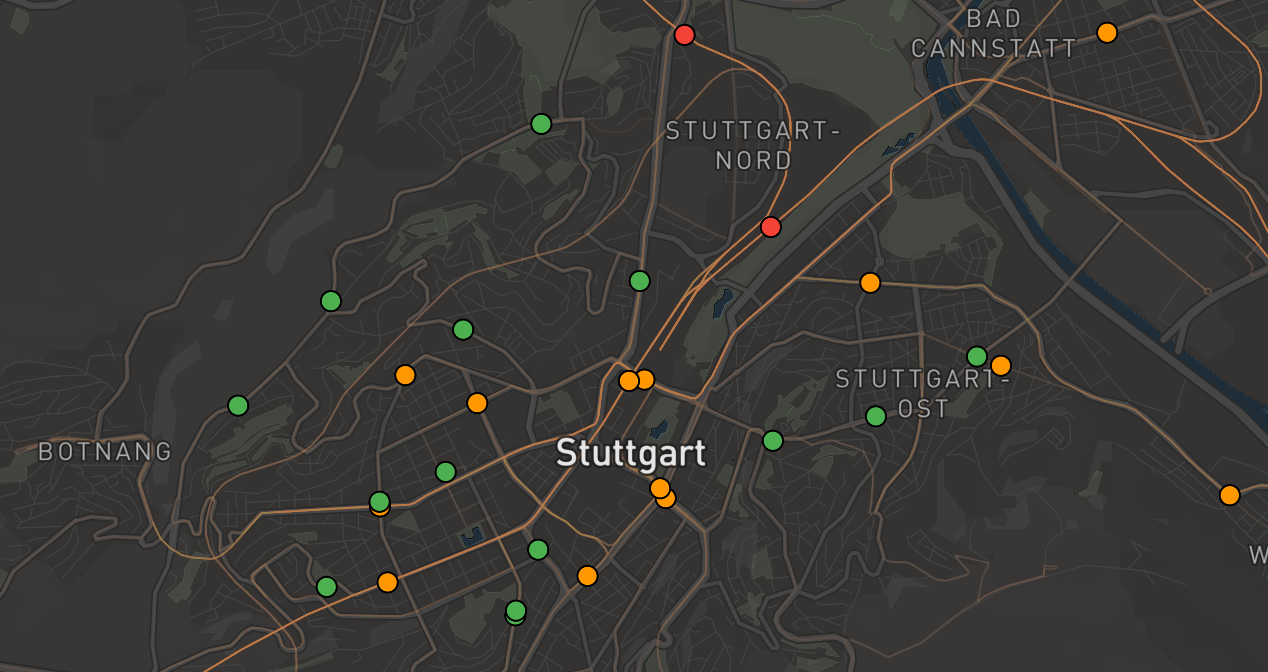
\includegraphics[width=0.6\textwidth]{map}
        \caption{Die Karte mit angepasstem Style: Mapbox-Dark}
        \label{fig:map}
      \end{center}
    \end{figure}
    
  % subsubsection die_karte (end)

  \subsubsection*{Vehicle}
  \label{ssub:vehicle}
    Die Vehicle sind auf der Karte als Kreis dargestellt. Die gegebene Farbe orientiert sich dabei an den öffentlichen Farben des Verkehrsunternehmens. Zum Beispiel sind Interrail Züge im Rot der Deutschen Bahn dargestellt und die U und S-Bahn hat das Orange von Stuttgart-VVS.\\

    Vehicle werden auf der Karte Animiert, wenn sie aktiv. Abbildung \ref{fig:vehicle_states} zeigt die zwei verschiedenen Animationen, die ein Vehicle beim Beginnen und Beendigen des Trips annehmen kann. Wird ein Trip aktiv, so wird das dazugehörende Vehicle auf die Karte platziert. Dabei ist der Radius des Vehicles verringert, bis er der Größe der anderen Vehicle entspricht.

    \begin{figure}[htbp]
      \centering
      \subfloat[Vehicle beginnt seinen Trip und wird aktiv]{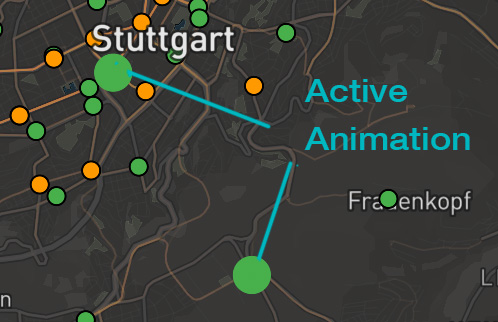
\includegraphics[width=0.34\textwidth]{vehicle_active.jpg}\label{fig:vehicle_active}}
      \hfill
      \subfloat[Vehicle beendet seinen Trip innerhalb von 30 Sekunden und wird inaktiv]{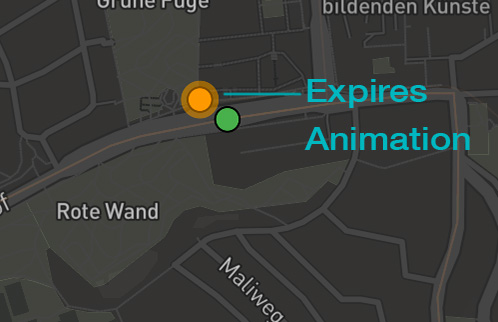
\includegraphics[width=0.34\textwidth]{vehicle_expires.jpg}\label{fig:vehicle_expires}}
      \caption{Vehicle Status Anzeige}
      \label{fig:vehicle_states}
    \end{figure}

    
    Ist ein Vehicle dabei seinen Trip innerhalb von 30 Sekunden zu beenden, so wird ein leicht transparentes Pulsieren angezeigt. Nachdem das Vehicle den Trip beendet hat, wird es von der Karte genommen und verschwindet. Technisch betrachtet werden erst alle Referenzen auf das Vehicle beseitigt und anschließend das Vehicle Objekt gelöscht.
    
  % subsubsection vehicle (end)

  \subsubsection*{Zeitstrahl}
  \label{ssub:zeitstrahl}
    Der Zeitstrahl in Abbildung \ref{fig:timeline} besteht aus mehreren Einzelteilen. 

    \begin{figure}[htbp]
      \begin{center}
        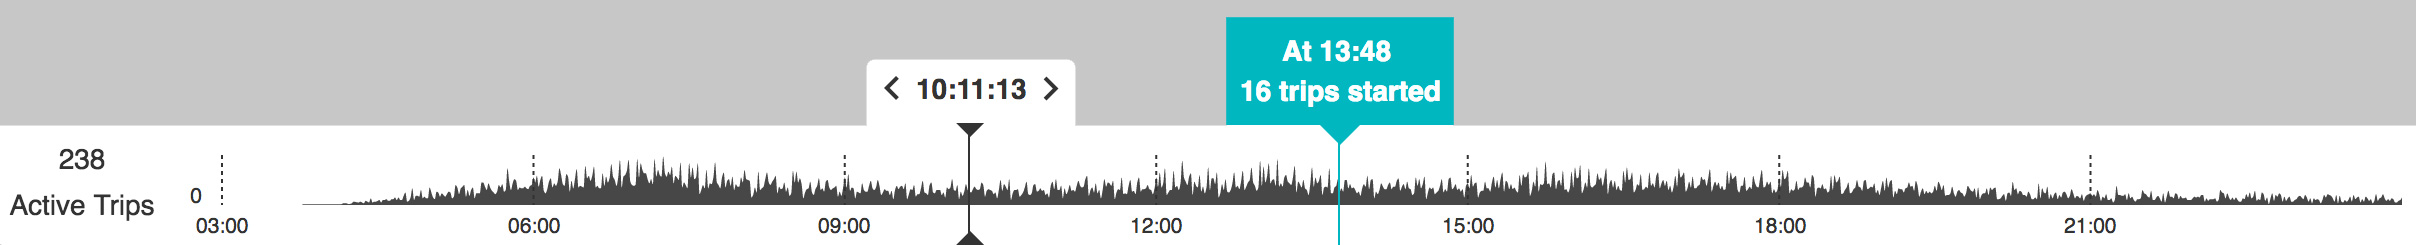
\includegraphics[width=\textwidth]{timeline}
        \caption{Zeitstrahl Komponente}
        \label{fig:timeline}
      \end{center}
    \end{figure}

    Links unten ist die Anzahl an momentan aktiven Trips zu sehen. Diese Anzahl korreliert mit den Vehicles auf der Karte. Die Anzeige wird immer aktuell gehalten und steigt, falls neue Trips aktiv werden, oder fällt wenn ein Trip beendet ist. Der Zeitstrahl selbst zeigt die Anzahl an aktiv werdenden Trips pro Minute an. Bewegt der Anwender die Maus darüber, so bekommt er die genaue Trip Anzahl zu einer Uhrzeit als Tooltip angezeigt. Ebenfalls ist es möglich die Animation zu einem beliebigem Zeitpunkt anzuzeigen. Dafür kann der Anwender einfach auf die gewünschte Zeitmarke im Zeitstrahl klicken und die Animation aktualisiert sich. Damit lässt sich die Karte zu unterschiedlichen Tageszeiten untersuchen. Zuletzt ist auch die gewählte Uhrzeit auf dem Zeitstrahl zu sehen. Diese zeigt dem Anwender, welcher Zeitpunkt momentan auf der Karte angezeigt wird.
    
  % subsubsection zeitstrahl (end)

  \subsubsection*{Filter}
  \label{ssub:filter}
    Über ein ausklappbares Menü, lassen sich verschiedene Filter auswählen. Dadurch kann der Anwender zum Beispiel alle Vehicle eines Typs oder einer Linie darzustellen. Auch Kombinationen der \texttt{Filter Vehicles} und \texttt{Filter Lines} sind möglich. Da aber meist eine Linie von genau einem Vehicle Typ bedient wird, macht das oft keinen Sinn.

    Damit der Anwender die Relation zwischen dem Filter und den Vehicle auf der Karte versteht, sind die Farben einheitlich gestaltet. Nachdem ein Filter ausgewählt ist, kann das Menü entweder wieder zugeklappt werden, oder der Filter lässt sich wieder abwählen.

    \begin{figure}[htbp]
      \begin{center}
        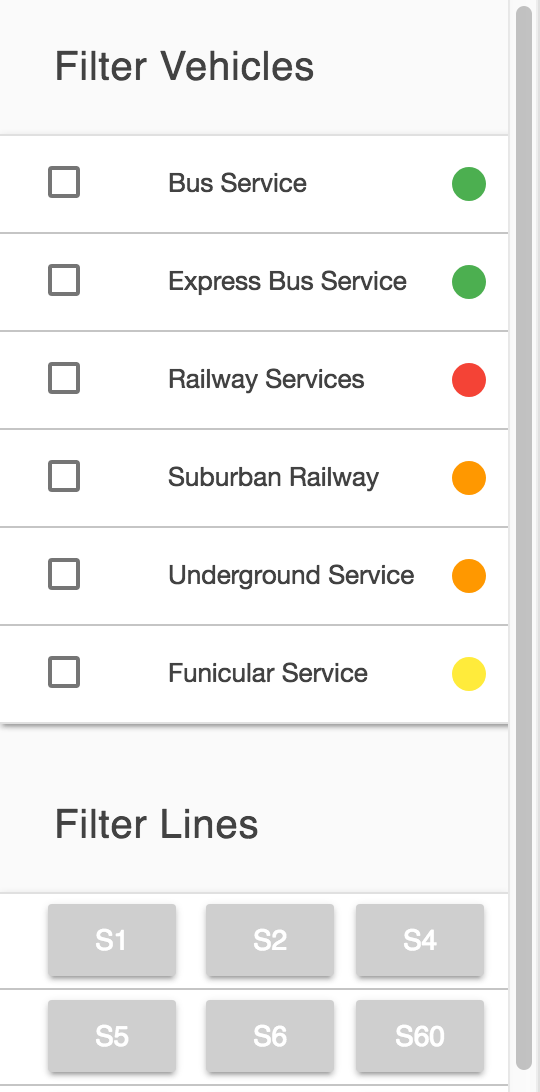
\includegraphics[width=0.2\textwidth]{filter}
        \caption{Filter Funktion}
        \label{fig:filter}
      \end{center}
    \end{figure}
    
  % subsubsection filter (end)

  \subsubsection*{Anzeigen von Trip Informationen}
  \label{ssub:anzeigen_von_trip_informationen}
    Wenn der Anwender ein Vehicle in der Karte durch Klicken auswählt, öffnet sich ein Fenster, welches Informationen für diesen Trip anzeigt (Abbildung \ref{fig:trip_information}. Neben dem Namen der Route lässt sich im Kreis (hier in Rot) die Routen Nummer ablesen. Im unteren Bereich sind die Fahrplaninformationen für den Trip gelistet. Neben dem Namen der Station ist auch die Abfahrtzeit des Vehicles gelistet. Die bereits besuchten Stationen werden in einem Grauton dargestellt um sie als inaktiv zu markieren.


    \begin{figure}[htbp]
      \begin{center}
        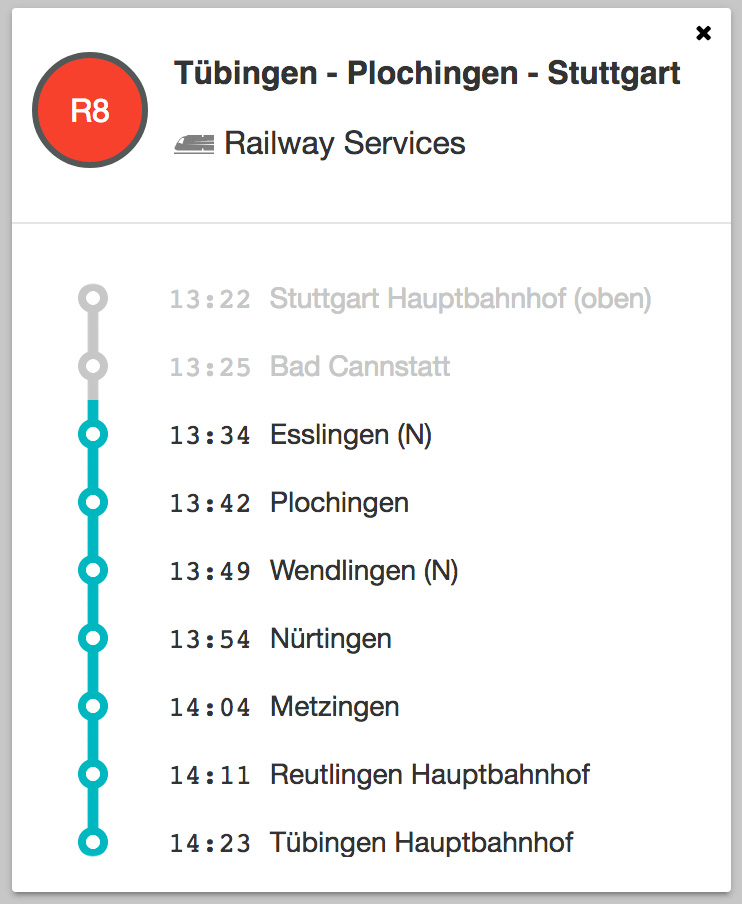
\includegraphics[width=0.3\textwidth]{trip_information}
        \caption{Anzeigen von Trip Informationen}
        \label{fig:trip_information}
      \end{center}
    \end{figure}

    \pagebreak
    
  % subsubsection anzeigen_von_trip_informationen (end)

  \subsubsection*{Wechseln der Kartendarstellung}
  \label{ssub:style_auswahl}
    Über das \texttt{Switch Style} \inlinegraphics{switch_styles_symbol} Element hat der Anwender die Möglichkeit zwischen verschiedenen Darstellungsarten der Karte zu wechseln. Auch die Polylines der Routen lassen sich zusätzlich über das Anwählen von \texttt{Shape} ein- oder ausblenden. Standardmäßig ist \texttt{Dark} ausgewählt.

    \begin{figure}[htbp]
      \begin{center}
        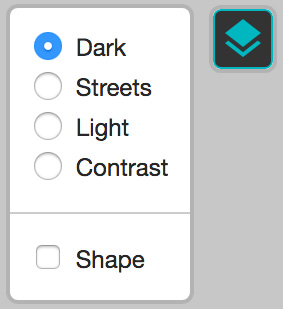
\includegraphics[width=0.14\textwidth]{switch_styles}
        \caption{Wechseln zwischen verschiedenen Kartendarstellung}
        \label{fig:switch_styles}
      \end{center}
    \end{figure}
    
  % subsubsection style_auswahl (end)

  \subsubsection*{Linien Finder}
  \label{ssub:linien_finder}
    Durch klicken des \texttt{Line Finder} \inlinegraphics{line_finder_symbol} Buttons lässt sich auf der Karte eine Route finden, die zwei Stationen $A, B$ verbindet. Dafür setzt der Anwender zwei Pins auf die Karte. Danach sucht ein Algorithmus diejenige Route aus, die am besten diese Stationen verbindet. Das Ergebnis sieht dann wie folgt aus:

    \begin{figure}[htbp]
      \begin{center}
        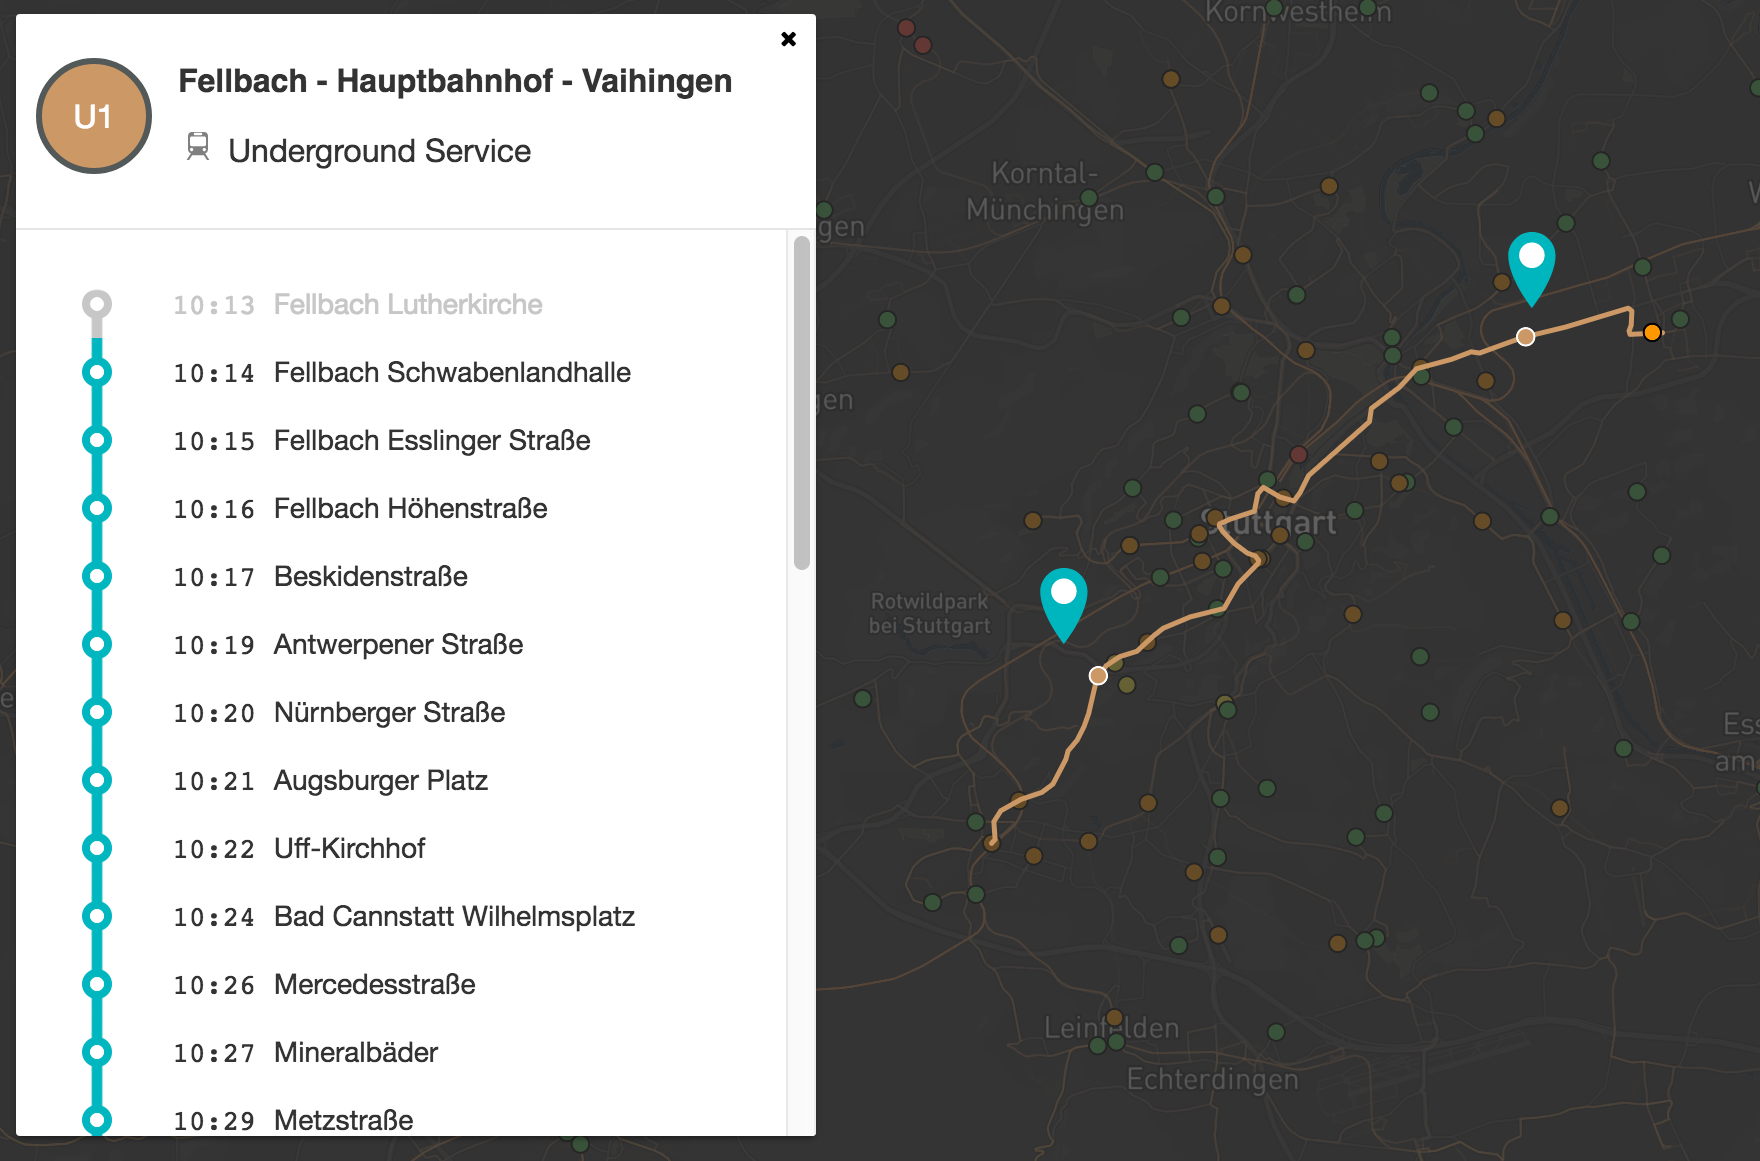
\includegraphics[width=0.6\textwidth]{line_finder}
        \caption{Linien Finder}
        \label{fig:line_finder}
      \end{center}
    \end{figure}

    Diese Funktion vereint Visualisierung und Wegfindung in einer Applikation. Während wir momentan ausschließlich eine Wegfindung über verschiedene Formularfelder (Von..., Nach..., Datum, Uhrzeit) beginnen, könnte es für städtische oder regionale Wegfindung auch eine visuelle Lösung geben. Der Vorteil liegt dabei, dass kein Kontextwechsel nötig ist. Die Orientierung, Wegfindung und Fahrplaninformationen ließen sich alle in einer Ansicht unterbringen. Ein weiteres Merkmal dieses visuellen Ansatzes ist die Möglichkeit eine Route zu finden, ohne dass die Namen der Haltestellen bekannt sein müssen. Das auf der Karte dargestellte Ergebnis, zeigt dem Nutzer auch gleich, wo sich das zur Route gehörende Vehicle sich befindet. Damit könnte der Anwender auch gleich entscheiden, ob er dieses Vehicle noch erreichen würde oder nicht. Dabei ließen sich auch sehr gut GTFS-Realtime Informationen verwenden, so dass man gleich sehen würde ob das Vehicle zum Beispiel Verspätung hat.\\

    Von allen implementierten Komponente hat der Linien Finder am meisten Potential für verschiedene Weiterentwicklungen. Angefangen von der Implementierung von Echtzeitinformationen, über eine integrierte Anwender Navigation (zum Beispiel könnte man den Anwender zu einer Station navigieren), als auch das Anbieten von Möglichkeiten zum Verbindungsanschluss wären möglich. Ebenfalls kann der Algorithmus zur Auswahl der empfohlenen Route noch sehr viel weiter verbessert werden. Momentan fließt vor allem die mittlere Distanz zwischen gesetztem Pin und nächster Station in die Entscheidung ein. Weitere Faktoren könnten aber noch berücksichtigt werden. Beispielsweise der Typ des Vehicles (U-Bahn bevorzugt gegenüber Bus), Frequenz der Route, Wartezeit auf das Vehicle, Preis, Reisezeit oder gar das momentane Verkehrsaufkommen.
    
  % subsubsection linien_finder (end)
  

  % * Timeline Component (Time jump + Trip counter, Trips that get active)
  % * Vehicles, Vehicle States (active, inactive)
  % * Filtering mechanism (Lines / Type)
  % * Layer switcher
  % * Route finder
  % * Bezier Easing 
  
% subsubsection ui_komponenten (end)


  % subsection frontend (end)

\end{newpage}

% section implementierung (end)
\end{newpage}
  \begin{newpage}
	% \hline
	\vspace*{\fill}
	\section*{Eidesstattliche Erklärung }
	Hiermit versichere ich, die vorliegende Arbeit selbstständig und unter ausschließlicher Verwendung der angegebenen Literatur und Hilfsmittel erstellt zu haben. Die Arbeit wurde bisher, in gleicher oder ähnlicher Form, keiner anderen Prüfungsbehörde vorgelegt und auch nicht veröffentlicht.\\

	\vspace{3cm}
	\begin{tabular*}{\textwidth}{c@{\extracolsep\fill}cc}
	\cline{1-1}
	\cline{3-3}
	\\
	\ \ \ \ \ \ \ \ \ Unterschrift \ \ \ \ \ \ \ \ \ \ & & \ \ \ \ \ \ \ \ \ Ort, Datum \ \ \ \ \ \ \ \ \ \\
	\end{tabular*}
\end{newpage}

\newpage
  
	\printbibliography

  \begin{newpage}
\section{Anhang}
\label{sec:anhang}

\begin{lstlisting}[captionpos=t, caption=Postgresql Datenbankabfrage von allen aktiven Trips mit ihrem dazugehörigen Linienverlauf, label=lst:get_active_trips_query, language=SQL]
SELECT 
  array_to_json(ARRAY_AGG(array[stop_lat, stop_lon])) AS stops_coords,
  array_to_json(ARRAY_AGG(array[
    CAST ( stops.stop_id AS TEXT ),
    CAST ( stop_times.stop_sequence AS TEXT ),
    stops.stop_name, 
    stop_times.departure_time,
    CAST ( stop_times.departure_time_seconds AS TEXT ),
    stop_times.arrival_time,
    CAST ( stop_times.arrival_time_seconds AS TEXT )
  ] ORDER BY stop_times.stop_sequence)) AS stops_object,
  routes.route_short_name,
  routes.route_long_name,
  routes.route_type,
  routes.route_color,
  routes.route_text_color,
  trips.trip_id, 
  trips.route_id,
  trips.direction_id,
  frequency.start_time, 
  frequency.end_time, 
  frequency.start_time_seconds,
  frequency.end_time_seconds,
  frequency.headway_secs AS frequency_seconds,
  calendar.start_date,
  calendar.end_date,
  agencies.agency_timezone,
  agencies.agency_id,
  agencies.agency_name,
  array_to_json(ARRAY_AGG(array[shape_pt_lat, shape_pt_lon] 
    ORDER BY shape_pt_sequence ASC)) AS shape_coords
FROM gtfs_stop_times AS stop_times

INNER JOIN gtfs_trips AS trips
  ON trips.trip_id = stop_times.trip_id 
  AND trips.agency_key = stop_times.agency_key
    
INNER JOIN gtfs_routes AS routes
  ON routes.route_id = trips.route_id 
  AND routes.agency_key = trips.agency_key
   
INNER JOIN gtfs_agency AS agencies
  ON agencies.agency_id = routes.agency_id 
  AND agencies.agency_key = routes.agency_key

INNER JOIN gtfs_stops AS stops 
  ON stops.stop_id = stop_times.stop_id
  AND stops.agency_key = stop_times.agency_key
  AND NOT EXISTS (
    SELECT 0
    FROM denormalized_max_stop_sequence AS max
    WHERE max.agency_key = stop_times.agency_key
    AND max.trip_id = stop_times.trip_id
    AND max.trip_max = stop_times.stop_sequence
  )

LEFT JOIN gtfs_calendar_dates AS calendar_dates
  ON calendar_dates.service_id = trips.service_id
  AND calendar_dates.agency_key = trips.agency_key
  AND date = '2017-05-10' 
  AND calendar_dates.exception_type = 1

LEFT JOIN gtfs_calendar AS calendar 
  ON trips.service_id = calendar.service_id
  AND calendar.agency_key = trips.agency_key
  AND calendar.thursday = 1
  AND '2017-05-10' BETWEEN calendar.start_date 
  AND calendar.end_date OR calendar_dates.date IS NOT NULL
  AND calendar.start_date <= '2017-05-10'
  AND calendar.end_date >= '2017-05-10'

LEFT JOIN gtfs_frequencies AS frequency
  ON frequency.trip_id = trips.trip_id
  AND frequency.agency_key = trips.agency_key
    
LEFT JOIN gtfs_shapes AS shapes
  ON trips.shape_id = shapes.shape_id
  AND trips.agency_key = shapes.agency_key

WHERE (
  frequency.start_time_seconds >= 25200 
  AND frequency.end_time_seconds <= 90000
  AND shapes.shape_id IS NOT NULL
  AND '2017-05-10' BETWEEN calendar.start_date 
  AND calendar.end_date OR calendar_dates.date IS NOT NULL
) 
AND NOT EXISTS (
  SELECT 0
  FROM gtfs_calendar_dates AS date_exceptions
  WHERE date = '2017-05-10'
  AND date_exceptions.agency_key = trips.agency_key
  AND date_exceptions.service_id = trips.service_id
  AND exception_type = 2
)
GROUP BY 
  routes.route_short_name,
  routes.route_long_name,
  routes.route_type,
  routes.route_color,
  routes.route_text_color,
  trips.trip_id, 
  trips.route_id,
  trips.direction_id,
  frequency.start_time, 
  frequency.end_time, 
  frequency.start_time_seconds,
  frequency.end_time_seconds,
  frequency_seconds,
  calendar.start_date,
  calendar.end_date,
  agencies.agency_timezone,
  agencies.agency_id,
  agencies.agency_name
\end{lstlisting}


\begin{lstlisting}[captionpos=t, caption=Erstellen einer denormalized\_shapes Tabelle, label=lst:sql_aggregate_shape, language=SQL]
-- first we creat the new database table
CREATE TABLE denormalized_shapes (
  agency_key text,
  shape_id INTEGER,
  shape_coords json,
  shape_dist_traveled double precision[]
);

-- generating indexes
CREATE INDEX denormalized_shapes_unique_index 
  ON denormalized_shapes (agency_key, shape_id);

-- insert the shape data into new table
INSERT INTO denormalized_shapes
SELECT
  agency_key,
  shape_id,
  shape_coords,
  shape_dist_traveled
FROM (
  SELECT
    shapes.agency_key,
    shapes.shape_id,
    array_to_json(ARRAY_AGG(array[shape_pt_lon, shape_pt_lat]
      ORDER BY shape_pt_sequence ASC))
      AS shape_coords,
    ARRAY_AGG(shape_dist_traveled
      ORDER BY shape_pt_sequence ASC)
      AS shape_dist_traveled

  FROM gtfs_shapes AS shapes

  GROUP BY
    shapes.agency_key,
    shapes.shape_id
) as shp;
\end{lstlisting}

\begin{lstlisting}[captionpos=t, caption=Erstellen der denormalized\_shapes Tabelle, label=lst:denormalized_shapes, language=SQL]
-- create denormalized_trips table
CREATE TABLE denormalized_trips (
  stops_coords json NOT NULL,
  stops_object json NOT NULL,
  stops_dist_traveled json,
  agency_key TEXT NOT NULL,
  trip_id INTEGER NOT NULL,
  route_id INTEGER NOT NULL,
  service_id INTEGER NOT NULL,
  shape_id INTEGER,
  trip_start_time INTEGER NOT NULL,
  trip_end_time INTEGER NOT NULL,
  direction_id INTEGER,
  route_color TEXT,
  route_long_name TEXT,
  route_short_name TEXT,
  route_desc TEXT,
  route_type INTEGER
);
-- create indexes
CREATE INDEX denormalized_trips_index 
  ON denormalized_trips (agency_key, trip_id, route_id, shape_id);
-- now query the data and insert it into the newly created table
INSERT INTO denormalized_trips
SELECT
  stops_coords,
  stops_object,
  agency_key,
  trip_id,
  route_id,
  service_id,
  shape_id,
  trip_start_time,
  trip_end_time,
  route_color,
  route_long_name,
  route_short_name,
  route_desc,
  route_type
FROM (
  SELECT
    array_to_json(ARRAY_AGG(array[stop_lat, stop_lon]
      ORDER BY stop_times.stop_sequence::int)) AS stops_coords,
    array_to_json(ARRAY_AGG(array[
        stops.stop_id,
        CAST ( stop_times.stop_sequence AS TEXT ),
        stops.stop_name,
        stop_times.departure_time,
        CAST ( stop_times.departure_time_seconds AS TEXT ),
        stop_times.arrival_time,
        CAST ( stop_times.arrival_time_seconds AS TEXT )
    ] ORDER BY stop_times.stop_sequence::int)) AS stops_object,
    trips.agency_key,
    trips.trip_id,
    trips.route_id,
    trips.service_id,
    trips.shape_id,
    min(stop_times.arrival_time_seconds) as trip_start_time,
    max(stop_times.departure_time_seconds) as trip_end_time,
    routes.route_color,
    routes.route_long_name,
    routes.route_short_name,
    routes.route_desc,
    routes.route_type
  FROM gtfs_stop_times AS stop_times

  INNER JOIN gtfs_trips AS trips
    ON trips.trip_id = stop_times.trip_id
    AND trips.agency_key = stop_times.agency_key

  INNER JOIN gtfs_routes AS routes
    ON trips.agency_key = routes.agency_key
    AND routes.route_id = trips.route_id

  INNER JOIN gtfs_stops AS stops
    ON stops.stop_id = stop_times.stop_id
    AND stops.agency_key = stop_times.agency_key

  GROUP BY
    trips.agency_key,
    trips.trip_id,
    trips.route_id,
    trips.service_id,
    trips.shape_id,
    routes.route_color,
    routes.route_long_name,
    routes.route_short_name,
    routes.route_desc,
    routes.route_type
) as trps;
\end{lstlisting}

\begin{lstlisting}[captionpos=t, caption=Abfrage von Trips und dessen Polyline in einer Zeitspanne XY zu einem gegebenen Datum Z, label=lst:query_trips, language=SQL]
SELECT
  trips.stops_coords,
  trips.stops_object,
  trips.stops_dist_traveled,
  shapes.shape_coords,
  trips.route_id,
  trips.shape_id,
  trips.trip_id,
  trips.route_color,
  trips.route_desc,
  trips.route_type,
  trips.route_long_name,
  trips.route_short_name,
  trips.trip_start_time,
  trips.trip_end_time
FROM denormalized_trips AS trips

INNER JOIN gtfs_calendar_dates AS calendar_dates
ON calendar_dates.service_id = trips.service_id
AND calendar_dates.agency_key = trips.agency_key
AND date = 'YYYY-MM-DD'
AND exception_type = 1

-- GTFS STUTTGART-VVS does not make use of the calendar, 
-- if you want to process other feeds aswell you might need
-- to join this table too
--LEFT JOIN gtfs_calendar AS calendar
--  ON trips.service_id = calendar.service_id
--  AND calendar.agency_key = trips.agency_key
--  AND calendar.$date = 1

LEFT JOIN denormalized_shapes AS shapes
  ON trips.shape_id = shapes.shape_id
  AND trips.agency_key = shapes.agency_key

WHERE (
  trip_start_time BETWEEN XY AND XY
  AND shapes.shape_coords IS NOT NULL
)
--AND (
--  'YYYY-MM-DD' BETWEEN calendar.start_date AND calendar.end_date
--  OR calendar_dates.date IS NOT NULL
--)
AND NOT EXISTS (
  SELECT 0
  FROM gtfs_calendar_dates AS date_exceptions
  WHERE date = 'YYYY-MM-DD'
  AND date_exceptions.agency_key = trips.agency_key
  AND date_exceptions.service_id = trips.service_id
  AND exception_type = 2
)
\end{lstlisting}
  

\begin{lstlisting}[captionpos=t, caption=Geojson FeatureCollection als Antwort zu \texttt{/trips/:from,:to}, label=lst:geojson_featurecollection]
{
  2498: {
    "type": "FeatureCollection",
    "features": [24]
  },
  1925: {
    "type": "FeatureCollection",
    "features": [7]
  },
  ...
}
\end{lstlisting}


\begin{lstlisting}[captionpos=t, caption=Shape Feature, label=lst:shape_feature,texcl=true, language=JavaScript, literate={ö}{{\"o}}1]
"features": [
  {
    "type": "Feature",
    "properties": {
      "name": "shape",
      "route_color": "#FF0000",
      "route_type": 700,
      "trip_id": 8784,
      "route_short_name": "701",
      "route_long_name": "Sindelf. Eichholz - ZOB - Böbl. ZOB - Diezenhalde",
      "trip_start": 55560,
      "trip_end": 57780,
      "route_type_color": "#f44336",
      "polyline": "kswv@}x`jH_@f@}@?c@UiJ{AQHiBeAqDcCl@yAjAoB|@iAjBsC^cAOi@yCsA
      _FgAq@MuB@_@YkAa@}A]cDgAUM_FLoa@qBcHq@T{@eCqD_EoDoNiJoJwIaGuHaDqGaCmM?cF|
      @kFvLoSxDaFlG{EpAkA\mAFcBf@q@vA_CO_B[
      m@DiB^eANgAG}APuAbAeARYRm@HyA@}ISyBEiAKsGDsCf]aBmBgP]
      iDDiBNsAtBs@~GiBrAm@tCyEzCqCdDyB~FmC|AWhEY|R]
      rHAxKDnFAdMFvc@lE~JtA|Ex@bD`@vKrBnG~@nDRdBDfONj]z@jKlA`DNvC@zGS|E_@`Dg@zF
      sAxHqAlCa@rDKzIB|FLM\?f@|Fv@dBvC|@\d@s@H_CjCPjA@pKLHqBF_GD_@"
    },
    "geometry": {
      "type": "LineString",
      "coordinates": []
    }
  }
]  
\end{lstlisting}

\begin{lstlisting}[captionpos=t, caption=Station Feature, label=lst:station_feature]
{
  "type": "Feature",
  "properties": {
    "stop_id": "4637",
    "stop_sequence": 1,
    "stop_name": "Sindelf. Eichholz",
    "departure_time_secs": "55560",
    "arrival_time_secs": "55560",
    "secs_between_stops": 60,
    "dist_traveled": 0,
    "delta_dist_traveled": 0
  },
  "geometry": {
    "type": "Point",
    "coordinates": [
      9.002212,
      48.73068
    ]
  }
}
\end{lstlisting}

\begin{lstlisting}[captionpos=t, caption=Station Matching, label=lst:match_station, language=JavaScript]
const _ = require('lodash');
const knn = require('rbush-knn');
const rbush = require('rbush');
const turf = require('turf');

// own implementation of turf.js pointOnLine()
// https://github.com/Turfjs/turf/tree/master/packages/turf-point-on-line
function getPointOnLine(line, pt, units) {
  let coords;

  if (line.type === 'Feature') {
    coords = line.geometry.coordinates;
  } else if (line.type === 'LineString') {
    coords = line.coordinates;
  } else {
    throw new Error('input must be a LineString Feature or Geometry');
  }

  let closestPt = turf.point([Infinity, Infinity], { dist: Infinity });
  const start = turf.point(coords[0]);
  const stop = turf.point(coords[1]);
  start.properties.dist = turf.distance(pt, start, units);
  stop.properties.dist = turf.distance(pt, stop, units);
  // perpendicular
  const heightDistance = Math.max(start.properties.dist, stop.properties.dist);
  const direction = turf.bearing(start, stop);
  const perpendicularPt1 = turf.destination(pt, heightDistance, direction + 90, units);
  const perpendicularPt2 = turf.destination(pt, heightDistance, direction - 90, units);
  const intersect = turf.lineIntersect(
    turf.lineString([perpendicularPt1.geometry.coordinates, perpendicularPt2.geometry.coordinates]),
    turf.lineString([start.geometry.coordinates, stop.geometry.coordinates]));
  let intersectPt = turf.point([Infinity, Infinity], { dist: Infinity });
  if (intersect.features.length > 0) {
    intersectPt = intersect.features[0];
    intersectPt.properties.index = line.properties.index1;
    intersectPt.properties.dist = turf.distance(pt, intersectPt, units);
  }

  if (start.properties.dist < closestPt.properties.dist) {
    closestPt = start;
    closestPt.properties.index = line.properties.index1;
  }
  if (stop.properties.dist < closestPt.properties.dist) {
    closestPt = stop;
    closestPt.properties.index = line.properties.index2;
  }
  if (intersectPt && intersectPt.properties.dist < closestPt.properties.dist) {
    closestPt = intersectPt;
    closestPt.properties.index = line.properties.index1;
  }
  return closestPt;
}

// own implementation of turf.js pointOnLine()
// https://github.com/Turfjs/turf/tree/master/packages/turf-line-slice
function lineSlice(startPt, stopPt, line) {
  const start = turf.point(startPt, { index: 0 });
  let coords;
  if (line.type === 'Feature') {
    coords = line.geometry.coordinates;
  } else if (line.type === 'LineString') {
    coords = line.coordinates;
  } else {
    throw new Error('input must be a LineString Feature or Geometry');
  }
  const ends = [stopPt, start];
  const clipCoords = [ends[0].geometry.coordinates];
  for (let i = ends[0].properties.index + 1; i < ends[1].properties.index + 1; i += 1) {
    clipCoords.push(coords[i]);
  }
  clipCoords.push(ends[1].geometry.coordinates);
  return turf.lineString(clipCoords, line.properties);
}

function fillTree(trips) {
  const tree = rbush(200, ['[0]', '[1]', '[0]', '[1]', '[2]']);
  const coords = [];
  for (let k = 0; k < trips.features[0].geometry.coordinates.length; k += 1) {
    const item = [
      trips.features[0].geometry.coordinates[k][0],
      trips.features[0].geometry.coordinates[k][1],
      { index: k },
    ];
    coords.push(item);
  }
  tree.load(coords);
  return tree;
}

function matchStation(geojson) {
  _.forEach(geojson, (trips) => {
    const shape = _.first(trips.features);
    for (let i = 1; i < trips.features.length; i += 1) {
      const tree = fillTree(trips);
      const lat = trips.features[i].geometry.coordinates[0];
      const lng = trips.features[i].geometry.coordinates[1];
      const neighbours = knn(tree, lat, lng, 2);
      const line = turf.lineString([
        [neighbours[0][0], neighbours[0][1]],
        [neighbours[1][0], neighbours[1][1]]],
        { index1: neighbours[0][2].index, index2: neighbours[1][2].index });
      const pointOnLine = getPointOnLine(line, trips.features[i], 'kilometers');
      const lineDistance = turf.lineDistance(lineSlice(trips.features[0].geometry.coordinates[0], pointOnLine, shape));
      trips.features[i].properties.dist_traveled = lineDistance * 1000;
      trips.features[i].geometry.coordinates = pointOnLine.geometry.coordinates;

      if (i > 1) {
        const deltaDist = trips.features[i].properties.dist_traveled - trips.features[i - 1].properties.dist_traveled;
        trips.features[i].properties.delta_dist_traveled = Math.abs(deltaDist);
      } else {
        trips.features[i].properties.delta_dist_traveled = 0;
      }
    }
  });
  return geojson;
}

\end{lstlisting}

      
\end{newpage}

\end{document}